\seccion{Unos ejemplos y aplicaciones}
\label{Sec:SZ:Ejemplos}


% ================================= canal

\subseccion{Canal de transmisi\'on y su capacidad}
\label{Ssec:SZ:CanalCapacidad}

Siguiendo el  esquema de comunicaci\'on de  Shannon, un mensaje  que se modeliza
como  un vector  aleatorio~\footnote{De  punto  de vista  de  un receptor,  este
  mensaje es  desconocido. Adem\'as, se lo  puede ver como una  instancia de una
  clase  importante   de  posibles  mensajes,   justificando  la  modelizaci\'on
  aleatoria.} $X$  pasa por un  canal de comunicaci\'on  y se recibe  un mensaje
$Y$, vector  aleatorio. En el trabajo de  Shannon, el canal es  supuesto a ruido
aditivo,  es decir  que se  a\~nade un  ruido a  $X$.  De  manera  general, para
conocer la informaci\'on de $X$ que se recibe, se calcula la informaci\'on mutua
$I(X;Y)$, es  decir la cantidad de  informaci\'on que comparten la  entrada y la
salida  del  canal.  Lo  m\'as  $I$  es grande,  lo  m\'as  de informaci\'on  se
transmite.  Dado el canal, se puede arreglar $X$ (su distribuci\'on) de manera a
maximizar $I(X;Y)$,  es decir  la cantidad m\'axima  que se puede  transmitir en
este    canal.    Es    lo     que    es    conocido    como    capacidad    del
canal~\cite[part.~II~\&~III]{Sha48} (ver  tambi\'en~\cite{CovTho06, Rio07} entre
otros):
%
\begin{definicion}[Capacidad de canal]
\label{Def:SZ:CapacidadCanal}
%
  Sea un canal de transmisi\'on, $X$  su entrada e $Y$ su salida, como ilustrado
  figura  Fig.~\ref{Fig:SZ:CanalComunicacion}.  Sea  $p_X$ la  distribuci\'on de
  probabilidad de $X$. La capacidad $C$ del canal es definida por
  %
  \[
  C = \max_{p_X} \, I(X;Y).
  \]
\end{definicion}

\begin{figure}[h!]
%
\begin{center} 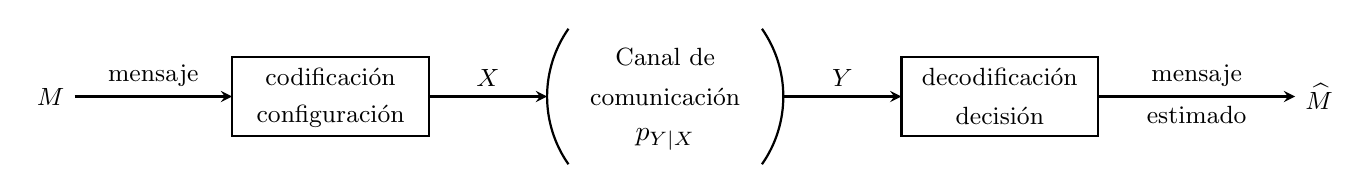
\begin{tikzpicture}
\shorthandoff{>}
%
% Mensaje
\draw[>=stealth,->,thick] (0,0) node[left]{\small $M$} --(2,0);
\draw (1,0) node[above]{\small mensaje};
%
% codificacion
\draw[thick] (2,-.5) rectangle (4.5,.5);
\draw (3.25,.25) node{\small codificaci\'on};
\draw (3.25,-.25) node{\small configuraci\'on};
%
% entrada del canal
\draw[>=stealth,->,thick] (4.5,0)--(6,0);
\draw (5.25,0) node[above]{\small $X$};
%
% Canal de com
\pgfmathsetmacro{\t}{35};
\pgfmathsetmacro{\r}{1.5};
\draw[thick] ({6+\r*(1+cos(180-\t))},{\r*sin(\t)}) arc (180-\t:180+\t:\r);
\draw[thick] ({6+\r*(1+cos(\t))},{-\r*sin(\t)}) arc (-\t:\t:\r);
\draw ({6+\r},.5) node{\small Canal de};
\draw ({6+\r},0) node{\small comunicaci\'on};
\draw ({6+\r},-.55) node{$p_{Y|X}$};
%
% salida
\draw[>=stealth,->,thick] ({6+2*\r},0)--({7.5+2*\r},0);
\draw ({6.75+2*\r},0) node[above]{\small $Y$};
%
% decodificacion/decision
\draw[thick] ({7.5+2*\r},-.5) rectangle ({10+2*\r},.5);
\draw ({8.75+2*\r},.25) node{\small decodificaci\'on};
\draw ({8.75+2*\r},-.25) node{\small decisi\'on};
%
% Mensaje estimado
\draw[>=stealth,->,thick] ({10+2*\r},0)--({12.5+2*\r},0) node[right]{\small $\widehat{M}$};
\draw ({11.25+2*\r},0) node[above]{\small mensaje};
\draw ({11.25+2*\r},0) node[below]{\small estimado};
\end{tikzpicture}
 \end{center}
%
\leyenda{Esquema de comunicaci\'on de Shannon.  En una primera etapa, un mensaje
  $M$ a  transmitir es  c\'odificado (ej.  c\'odigo  binario) o puesto  en forma
  (ej.  s\'imbolos  modulando una  funci\'on para que  sea anal\'ogica y  en una
  banda frecuencial dada).   Sea $X$ este mensaje codificado  o puesto en forma.
  A la  recepci\'on, se mide $Y$ (ej.   versi\'on ruidosa de $X$),  antes de ser
  decodificado  o  usado para  tomar  una  decisi\'on,  $\widehat{M}$ siendo  la
  estimaci\'on de  $M$ (ej.  s\'imbolos estimados  a partir de  $Y$).  Una etapa
  importante es el v\'inculo entre la entrada  $X$ y la salida $Y$ del canal, es
  decir la  cantidad de informaci\'on que  tienen en com\'un.   La capacidad del
  canal es la informaci\'on $I(X;Y)$ m\'axima con respeto a su entrada.}
\label{Fig:SZ:CanalComunicacion}
\end{figure}


% ================================= canal binario

\subsubseccion{Canal binario}
\label{Sssec:SZ:CanalBinario}

Suponiendo  que el  mensaje mandado  en un  canal es  una cadena  de s\'imbolos,
variables   aleatorias  independientes,   se  puede   concentrarse   sobre  cada
s\'imbolo. En este marco, un canal de comunicaci\'on lo m\'as simple es conocido
como  {\it canal  binario}~\cite[Sec.~15]{Sha48}: $X$  es una  variable definida
sobre  $\X =  \{ 0  , 1  \}$;  tal tipo  de entrada  es natural,  pensando a  la
codificaci\'on  binaria.  La  salida $Y$  es tambi\'en  definida sobre  $\X$; se
puede imaginar medir y tomar una decisi\'on binaria usando la medida.  Tal canal
es  definido por  sus  probabilidaded de  transici\'on  $p_{Y|X=x}(y)$, \ie  las
probabilidades que un 0 (resp. un 1) se transmite correctamente o cambia en un 1
(resp. 0), \ie
%
\[
\varepsilon = PY = 1 | X = 0) = 1 - P(Y = 0 | X = 0) \qquad \mbox{y} \qquad
\vartheta = P(Y = 0 | X = 1) = 1 - P(Y = 1 | X = 1).
\]
%
$\varepsilon$ y $\vartheta$ representan errores de comunicaci\'on.  Tal canal es
descrito      figura     Fig.~\ref{Fig:SZ:CanalBinario}-(a).       La     figura
Fig.~\ref{Fig:SZ:CanalBinario}-(b) da un esquema ``pr\'actico'' que podr\'ia ser
al origen  de un  tal canal.  Cuando  \ $\varepsilon  = \vartheta$, el  canal es
conocido como {\it canal binario sim\'etrico}.  Cuando \ $\varepsilon = 0$ \ y \
$\vartheta \in (0 \,  ; \, 1)$, el canal es conocido  como {\it canal binario en
  Z}.

\begin{figure}[h!]
\begin{center} 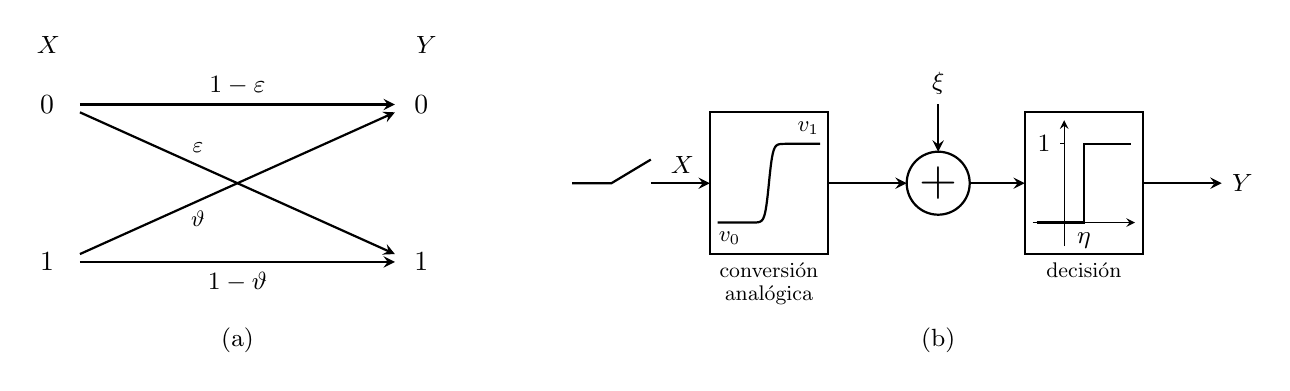
\begin{tikzpicture}
\shorthandoff{>}
%
\begin{scope}
\draw (-.4,1.75) node {\small $X$}; \draw (4.4,1.75) node {\small $Y$};
%
\draw[>=stealth,->,thick] (-.2,1) node[left]{0} (0,1) -- (4,1) node[right]{\ 0};
\draw (2,1) node[above]{\small $1-\varepsilon$};
%
\draw[>=stealth,->,thick] (-.2,-1) node[left]{1} (0,-1) -- (4,-1) node[right]{\ 1};
\draw (2,-1) node[below]{\small $1-\vartheta$};
%
\draw[>=stealth,->,thick] (0,.9)--(4,-.9);
\draw (1.5,.45) node[scale=.9]{\small $\varepsilon$};
%
\draw[>=stealth,->,thick] (0,-.9)--(4,.9);
\draw (1.5,-.45) node[scale=.9]{\small $\vartheta$};
%
\end{scope}
%
\begin{scope}[xshift=7cm]
%
% entrada
\draw[thick] (-.75,0)--(-.25,0)--(.25,.3);
\draw[>=stealth,->,thick] (.25,0)--(1,0);
%\draw[>=stealth,->,thick] (.25,-.5) node[below]{\small $X$} --(.25,.1);
\draw (.65,0) node[above]{\small $X$};
%
% puesta en niveles
\draw[thick] (1,-.9) rectangle (2.5,.9);
\draw (1.25,-.7) node[scale=.9]{\small $v_0$};
\draw (2.25,.7) node[scale=.9]{\small $v_1$};
\draw[thick,domain=-4.5:4.5,samples=100] (1.1,-.5) -- plot ({\x/10+1.75},{.5*tanh(2*\x)}) --(2.4,.5);
\draw (1.75,-.9) node[below,scale=.85]{\small conversi\'on};
\draw (1.75,-1.2) node[below,scale=.85]{\small anal\'ogica};
%
% adicion del ruido
\draw[>=stealth,->,thick] (2.5,0)--(3.5,0);
\draw[thick] (3.9,0) circle (.4);
\draw[>=stealth,->,thick] (3.9,1) node[above]{\small $\xi$} --(3.9,.4);
\draw (3.9,0) node[align=center,scale=1.5]{\large +};
%
% decision
\draw[>=stealth,->,thick] (4.3,0)--(5,0);
\draw[thick] (5,-.9) rectangle (6.5,.9);
\draw[>=stealth,->] (5.1,-.5)--(6.4,-.5);
\draw[>=stealth,->] (5.5,-.8)--(5.5,.8);
\draw[thick] (5.15,-.5)--(5.75,-.5)--(5.75,.5)--(6.35,.5);
\draw (5.75,-.5) node[below]{\small $\eta$};
\draw (5.5,.5)--(5.45,.5) node[left]{\small 1};
\draw (5.75,-.9) node[below,scale=.85]{\small decisi\'on};
%
% salida
\draw[>=stealth,->,thick] (6.5,0)--(7.5,0) node[right]{\small $Y$};
\end{scope}
\draw (2,-2) node {\small (a)};
\draw (10.9,-2) node {\small (b)};
\end{tikzpicture}
 \end{center}
%
\leyenda{(a): Canal  binario. La entrada  $X$ definida sobre  $\X = \{ 0  , 1\}$
  pasa por este canal e $Y$ definida  sobre $\Y = \X$ es recibido. Este canal es
  caracterizado  por las  probabilidades de  transici\'on  $p_{Y|X=x}(y)$.  (b):
  Esquema que puede conducir al canal  binario; una variable puede ser la salida
  de una puerta l\'ogica, con niveles  $v_0$ (nivel bajo, codificando 0) y $v_1$
  (nivel  alto,  codificando  1).   Se   puede  imaginar  que  este  voltaje  es
  transmitido por un  canal a\~nandiendo un ruido $\xi$.   En la recepci\'on, se
  toma una  decisi\'on, por ejemplo  0 (resp.  1)  si la medida es  mayor (resp.
  menor)  que  $\eta  =   \frac{v_0  +  v_1}{2}+\Esp[\xi]$.   En  este  ejemplo,
  $\varepsilon$ \ y  \ $\vartheta$ \ van a  ser caracterizados completamente por
  la distribuci\'on  del ruido (y  de los dos  niveles posibles de  la entrada),
  pero no de la distribuci\'on $p_X$.}
\label{Fig:SZ:CanalBinario}
\end{figure}

En este caso, trabajando con bits, aparece leg\'itimo usar el logaritmo de base
2. Luego, sean
%
\[
r = P(X = 0),
\]
%
dando la distribuci\'on  de la entrada. La distribuci\'on de la  salida va a ser
dada a partir de $s = P(Y = 0) = P(Y = 0 | X = 0) P(X = 0) + P(Y = 0 | X
= 1) P(X = 1)$ es decir
%
\[
s = P(Y  = 0) = \vartheta +  r (1-\varepsilon-\vartheta).
\]
%
La informaci\'on  mutua se escribe  \ $I_2(X;Y) =  H_2(Y) - H_2(Y|X) =  H_2(Y) -
H_2(Y|X=0) P(X = 0) + H_2(Y|X=1) P(X = 1)$, lo que toma la expresi\'on
%
\[
I_2(X;Y) = h_2(s) - r h_2(\varepsilon) - (1-r) h_2(\vartheta),
\]
%
donde $h_2(u) = -  u \log_2 u - (1-u) \log_2 (1-u)$  es la entrop\'ia binaria en
bits.  Para calcular la capacidad $C_2$  en bits, hace falta maximizar $I_2$ con
respeto   a   $r$.    Diferenciando    $I_2$   en   $r$,   \ie   $\frac{\partial
  I_2(X;Y)}{\partial  r}  =  \frac{\partial h_2(s)}{\partial  s}  \frac{\partial
  s}{\partial r} - h_2(\varepsilon) + h_2(\vartheta)$, es decir
%
\[
\frac{\partial I_2(X;Y)}{\partial  r} = (1-\varepsilon-\vartheta)  \log_2 \left(
  \frac{1-s}{s} \right) - h_2(\varepsilon) + h_2(\vartheta).
\]
%
\begin{itemize}
\item Claramente,
  %
  \[
  \vartheta = 1-\varepsilon \quad \Rightarrow \quad C_2 = 0.
  \]
  %
  Viene del hecho de que  para $\vartheta = 1-\varepsilon$, de $h_2(\varepsilon)
  = h_2(1-\varepsilon)$  se deduce  que $I_2(X;Y) =  0$ constante. De  hecho, en
  este  caso, un 0  en la  salida puede  venir de  un 0  o 1  con probabilidades
  iguales, y  lo mismo para un  1 en la  salida; en otros t\'erminos,  la salida
  aparece ser independiente de la entrada.  Eso se verifica formalmente con $s =
  \vartheta$, dando  $p_{Y|X=x} =  p_Y$, dando una  informaci\'on mutua  nula, y
  entonces una capacidad nula.
%
\item Si $\vartheta  \ne 1-\varepsilon$, la derivada de $I_2$  con respeto a $r$
  se anula para $s = s^\opt$ ($r = r^\opt$),
  %
  \[
  s^\opt = \frac{1}{1 +  2^{\frac{h(\varepsilon) - h(\vartheta)}{1 - \varepsilon
        -  \vartheta}}}  \qquad \mbox{siendo}  \qquad  r^\opt  = \frac{s^\opt  -
    \vartheta}{1 - \varepsilon - \vartheta},
  \]
  %
  y  dando   un  extremo   para  $I_2$.   A   continuaci\'on,  $\frac{\partial^2
    I_2}{\partial  r^2} = \frac{(1-\varepsilon-\vartheta)^2}{s  (1-s)} >  0$ (en
  particular  para  el $s$  ``\'optimo''),  probando de  que  el  extremo es  un
  m\'aximo.  Poniendo  la expresi\'on de  $r^\opt$ en la formula  de $I_2(X;Y)$,
  luego de muchos c\'alculos (b\'asicos), se obtiene
  %
  \[
  C_2  =  \log_2\left(  1  +  2^{\frac{h_2(\varepsilon)  -  h_2(\vartheta)}{1  -
        \varepsilon   -  \vartheta}}   \right)  -   \frac{(1  -   \vartheta)  \,
    h_2(\varepsilon)  -   \varepsilon  \,  h_2(\vartheta)}{1   -  \varepsilon  -
    \vartheta}.
  \]
  %
  Cuando  $\vartheta   \to  1-\varepsilon$,  notando   que  $h_2(\varepsilon)  =
  h_2(1-\varepsilon)$ y  tomando el  l\'imite de esta  formula, se  recupera que
  $C_2 \to 0$.
  %
  % ---
  %
  % \newline{\color{red}\bf �Interpretacion?  no hay combinacion convexa
  %   $\frac{\varepsilon}{1-\varepsilon-\vartheta}$ siendo del mismo signo que
  %   $\frac{1-\vartheta}{1-\varepsilon-\vartheta}$; nota: $C
  %   = \log_2\left( 1 + 2^{-
  %       \frac{h(1-\vartheta)-h(\varepsilon)}{(1-\vartheta)-\varepsilon}}
  %   \right) + \frac{1}{\varepsilon
  %     (1-\vartheta)} \frac{(1-\vartheta) h(1-\vartheta) - \varepsilon
  %     h(\varepsilon)}{\vartheta - (1-\varepsilon)}$}
\end{itemize}
%
\noindent De  \ $I_2(X;Y) = H_2(Y)  - H_2(Y|X) \le H_2(Y)  \le 1$ bit  \ ($Y$ es
binario, de entrop\'ia m\'axima en el caso uniforme), aparece sin c\'alculos que
%
\[
C_2 \le 1 \: \mbox{bit},
\]
%
\ie la capacidad es menor que 1 bit~\footnote{De manera general, de la escritura
  de $I$ con entrop\'ias condicionales, para $X$ definido sobre $\X$ e $Y$ sobre
  $\Y$, da  \ $0 \le C \le  \min( \log |\X| \,  , \, \log |\Y|  )$.  \ Adem\'as,
  $p_{Y|X=x}$ depende solo del canal y no de la entrada, as\'i que para \ $p_X =
  \pi_1 p_{(1)} + \pi_2 p_{(2)}$ \ ($\pi_2 = 1-\pi_1$) se obtiene \ $p_Y = \pi_1
  q_{(1)}  + \pi_2  q_{(2)}$ \  con \  $q_{(i)}$ \  distribuci\'on de  la salida
  corespondiente a una entrada de distribuci\'on \ $p_{(i)}$.  Ahora, de $I(X;Y)
  = H(Y)-H(Y|X)$,  el segundo t\'ermino siendo dependiente  solamente del canal,
  de la  concavidad de  $H$ se  obtiene de que  $I$ es  c\'oncava con  respeto a
  $p_X$.  A continuaci\'on,  $p_X$  parteneciendo  a un  convexo,  $I$ tiene  un
  m\'aximo que es  \'unico.}: para transmitir informaci\'on en  este canal, hace
falta introducir redundancia en el mensaje.  Se  alcanza \ $C_2 = 1$ bit si, (i)
por  un  lado   $H_2(Y|X)  =  0$,  es  decir  \   $r  h_2(\varepsilon)  +  (1-r)
h_2(\vartheta) = 0$ \ y adem\'as (ii) \ $h_2(s) = 1$.  Estudiando cada caso (ej.
con \ $r = 0$ \ y \ $\vartheta =  0$ \ se satisface (i) pero no (ii) porque \ $s
= 0$), se obtiene que
%
\[
C_2  =  1  \qquad  \Leftrightarrow  \qquad  r =  \frac12  \quad  \mbox{y}  \quad
\varepsilon = \vartheta = \frac{1 \pm 1}{2}.
\]
%
Para  $\varepsilon =  \vartheta =  0$ el  canal es  perfecto, mientras  que para
$\varepsilon =  \vartheta =  1$ el  canal es llamado  {\it canal  volteando}; en
ambos casos, se recupera la entrada (o directamente, o tomando el opuesto) ``sin
perdida''.

La  figura  Fig.~\ref{Fig:SZ:ICanalBinario}  representa la  informaci\'on  mutua
$I(X;Y)$ para unos  canales ($\varepsilon$ y $\vartheta$ dados)  en funci\'on de
$r$.   Se nota que  la curva  es c\'oncava  y tiene  un m\'aximo,  capacidad del
canal.   La figura Fig.~\ref{Fig:SZ:CCanalBinario}  representa la  capacidad del
canal en  funci\'on de \  $\varepsilon$ \ y  \ $\vartheta$ as\'i que  unos casos
particulares/cortes.

En  el caso  particular  $\varepsilon  = \vartheta$,  conocido  como {\it  canal
  sim\'etico}, la capacidad es
%
\[
C_2 = 1 - h_2(\varepsilon)
\]
%
(alcanzada  con  una entrada  uniforme).   Como visto  en  el  caso general,  la
capacidad vale 1  bit si y solamente si  \ $h_2(\varepsilon) = 0$, \  es decir \
$\varepsilon = 0$ \ o \ $\varepsilon = 1$.  Al rev\'es, la capacidad es m\'inima
cuando $H_2$ est m\'aximo, es decir  para \ $\varepsilon = \vartheta = \frac12$,
\ y  \ $C_2 = 0$  \ (instancia particular  de \ $\vartheta =  1-\varepsilon$). \
$h_2(\varepsilon)$  \  es la  perdida  en bit  para  cada  bit transmitido.   La
capacidad  \  $C_2$   \  en  funci\'on  de  \   $\varepsilon$\  es  dada  figura
Fig.~\ref{Fig:SZ:CCanalBinario}-(b).

En el  caso particular  $\varepsilon = 0$,  conocido como  {\it canal en  Z}, la
capacidad es
%
\[
C_2 = \log_2\left( 1 +  2^{- \frac{h_2(\vartheta)}{1-\vartheta}} \right).
\]
%
Se nota  en este caso tambi\'en  que la capacidad  alcanza 1, su m\'aximo,  si y
solamente  si \  $\vartheta  = 0$  \  (canal perfecto).   Al  rev\'es, cuando  \
$\vartheta  \to 1$,  \  $C \to  0$, \  instancia  particular de  \ $\vartheta  =
1-\varepsilon$.   La capacidad \  $C_2$ \  en funci\'on  de $\vartheta$  es dada
figura Fig.~\ref{Fig:SZ:CCanalBinario}-(c).

%{\bf\color{red} C parecido a la de Shannon caso continuo. Interpretacion?}

\begin{figure}[h!]
%
\begin{center} \begin{tikzpicture}[scale=2]
\shorthandoff{>}
%
%
% ----- Canal general
%
\begin{scope}
\pgfmathsetmacro{\p}{.4};% varepsilon
\pgfmathsetmacro{\q}{.01};% vartheta
%
\pgfmathsetmacro{\dpr}{1-\p-\q};
\pgfmathsetmacro{\hp}{-\p*log2(\p)-(1-\p)*log2(1-\p)};% h(varepsilon)
\pgfmathsetmacro{\hq}{-\q*log2(\q)-(1-\q)*log2(1-\q)};% h(vartheta)
\pgfmathsetmacro{\dh}{\hp-\hq};
%
\pgfmathsetmacro{\bopt}{1/(1+(2^((\hp-\hq)/\dpr)))};% s opt
\pgfmathsetmacro{\aopt}{(\bopt-\q)/\dpr};% r opt
\pgfmathsetmacro{\Capa}{-log2(\bopt)-((1-\q)*\hp-\p*\hq)/\dpr};
%
\draw[>=stealth,->] (-.2,0)--(1.2,0) node[right]{\small $r$};
\draw[>=stealth,->] (0,-.2)--(0,1.2) node[above]{\small $I_2(X;Y)$};
%
\draw[thick,domain=0:1,samples=100] (0,0)-- plot (\x,
{-(\q+\dpr*\x)*log2(\q+\dpr*\x)-(1-\q-\dpr*\x)*log2(1-\q-\dpr*\x)-\x*\hp-(1-\x)*\hq)})
--(1,0);
%
\draw (\aopt,0)--(\aopt,-.05) node[below]{\small $r^\opt$};
\draw (1,0)--(1,-.05) node[below]{\small 1};
\draw (0,\Capa)--(-.05,\Capa) node[left]{\small $C_2$};
\draw (0,1)--(-.05,1) node[left]{\small 1};
\end{scope}
%
%
% ----- Canal simetrico
%
\begin{scope}[xshift=2.5cm]
\pgfmathsetmacro{\p}{.05};
%
\pgfmathsetmacro{\dpr}{1-2*\p};
\pgfmathsetmacro{\hp}{-\p*log2(\p)-(1-\p)*log2(1-\p)};
%
\pgfmathsetmacro{\Capa}{1-\hp};
%
\draw[>=stealth,->] (-.2,0)--(1.2,0) node[right]{\small $r$};
\draw[>=stealth,->] (0,-.2)--(0,1.2) node[above]{\small $I_2(X;Y)$};
%
\draw[thick,domain=0:1,samples=100] (0,0)-- plot (\x,
{-(\p+\dpr*\x)*log2(\p+\dpr*\x)-(1-\p-\dpr*\x)*log2(1-\p-\dpr*\x)-\hp)})
--(1,0);
%
\draw (.5,0)--(.5,-.05) node[below]{\small $r^\opt$};
\draw (1,0)--(1,-.05) node[below]{\small 1};
\draw (0,\Capa)--(-.05,\Capa) node[left]{\small $C_2$};
\draw (0,1)--(-.05,1) node[left]{\small 1};
\end{scope}
%
%
% ----- Canal en Z
%
\begin{scope}[xshift=5cm]
\pgfmathsetmacro{\q}{.3};
%
\pgfmathsetmacro{\dpr}{1-\q};
\pgfmathsetmacro{\hq}{-\q*log2(\q)-(1-\q)*log2(1-\q)};
%
\pgfmathsetmacro{\bopt}{1/(1+(2^(-\hq/\dpr)))};
\pgfmathsetmacro{\aopt}{(\bopt-\q)/\dpr};
\pgfmathsetmacro{\Capa}{-log2(\bopt)};
%
\draw[>=stealth,->] (-.2,0)--(1.2,0) node[right]{\small $r$};
\draw[>=stealth,->] (0,-.2)--(0,1.2) node[above]{\small $I_2(X;Y)$};
%
\draw[thick,domain=0:1,samples=100] (0,0)-- plot (\x,
{-(\q+\dpr*\x)*log2(\q+\dpr*\x)-(1-\q-\dpr*\x)*log2(1-\q-\dpr*\x)-(1-\x)*\hq)})
-- (1,0);
%
\draw (\aopt,0)--(\aopt,-.05) node[below]{\small $r^\opt$};
\draw (1,0)--(1,-.05) node[below]{\small 1};
\draw (0,\Capa)--(-.05,\Capa) node[left]{\small $C_2$};
\draw (0,1)--(-.05,1) node[left]{\small 1};
\end{scope}
\node at  (.5,-.6){\small (a)};
\node at  (3,-.6){\small (b)};
\node at  (5.5,-.6){\small (c)};
\end{tikzpicture}
 \end{center}
%
\leyenda{Informaci\'on mutua  (en bits) entrada-salida \ $I_2(X;Y)$  \ del canal
  binario en funci\'on de \ $r = P(X  = 0)$.  \ (a): \ $\varepsilon = 0.4$ \ y
  \  $\vartheta = 0.01$;  \ (b):  \ $\varepsilon  = \vartheta  = 0.05$  \ (canal
  sim\'etico); \ (c): \  $\varepsilon = 0$ \ y \ $\vartheta  = 0.05$ \ (canal en
  Z).}
%
\label{Fig:SZ:ICanalBinario}
\end{figure}

\

\begin{figure}[h!]
%
\begin{center} \begin{tikzpicture}[scale=2]
\shorthandoff{>}
%
%
% ----- Canal general
%
\begin{scope}
% C(\varepsilon,\vartheta)
%\begin{axis}[colorbar,domain=.01:.99, domain y=.01:.99, samples=10,  samples y=10,
%view={0}{90},  colormap/blackwhite,
%xlabel={\small $\varepsilon$}, ylabel={\small $\vartheta$}, xscale=.27, yscale=.27]
%\addplot3[surf,patch to triangles,shader=interp]
%%{5*sin(deg(2*pi*x))*exp(-4*pi*pi*y)};
%{log2(1+2^((-\x*log2(\x)-(1-\x)*log2(1-\x)+\y*log2(\y)+(1-\y)*log2(1-\y))/(1-\x-\y)))
%+((1-\y)*(\x*log2(\x)+(1-\x)*log2(1-\x))-\x*(\y*log2(\y)+(1-\y)*log2(\y)))/(1-\x-\y)};
%\end{axis}
%\draw(0,0) node{\color{red}\bf A faire};
\draw(1,.75) node{
\includegraphics[width=4cm]{TIKZ_SZ/CapacidadBinaria}};
\draw[>=stealth,->] (-.1,0)--(1.7,0) node[below]{\small $\varepsilon$};
\draw[>=stealth,->] (0,-.1)--(0,1.7) node[left]{\small $\vartheta$};
\draw (1.5,0)--(1.5,-.05) node[below,scale=.8]{\small 1};
\draw (0,1.5)--(-.05,1.5) node[left,scale=.8]{\small 1};
%
\draw (2.075,.02) node[scale=.8]{\small 0};
\draw (2.075,1.48) node[scale=.8]{\small 1};
\end{scope}
%
%
% ----- Canal simetrico
%
\begin{scope}[xshift=3.2cm,scale=1.3]
%
\draw[>=stealth,->] (-.1,0)--(1.2,0) node[right]{\small $\varepsilon$};
\draw[>=stealth,->] (0,-.1)--(0,1.2) node[above]{\small $C_2$};
%
\draw[thick,domain=.01:.99,samples=100] (0,1)-- plot (\x,
{1+\x*log2(\x)+(1-\x)*log2(1-\x)})
--(1,1);
%
\draw (.5,.75) node[scale=.8]{\small $(\vartheta = \varepsilon)$};
\draw (1,0)--(1,-.05) node[below,scale=.8]{\small 1};
\draw (0,1)--(-.05,1) node[left,scale=.8]{\small 1};
\end{scope}
%
%
% ----- Canal en Z
%
\begin{scope}[xshift=6cm,scale=1.3]
%
\draw[>=stealth,->] (-.2,0)--(1.2,0) node[right]{\small $\vartheta$};
\draw[>=stealth,->] (0,-.2)--(0,1.2) node[above]{\small $C_2$};
%
\draw[thick,domain=.01:.99,samples=100] (0,1)-- plot (\x,
{log2(1+2^(log2(1-\x)+(\x/(1-\x))*log2(1-\x)))})
-- (1,0);
%
\draw (.75,.75) node[scale=.8]{\small $(\varepsilon = 0)$};
\draw (1,0)--(1,-.05) node[below,scale=.8]{\small 1};
\draw (0,1)--(-.05,1) node[left,scale=.8]{\small 1};
\end{scope}
\draw (.8,-.4) node {\small (a)};
\draw (3.85,-.4) node {\small (b)};
\draw (6.75,-.4) node {\small (c)};
\end{tikzpicture}
 \end{center}
%
\leyenda{Capacidad  \ $C_2$ \  del canal  binario. \  (a): \  en funci\'on  de \
  $\varepsilon$ \  y \ $\vartheta$. \ (b):  \ en funci\'on de  \ $\varepsilon$ \
  para el canal sim\'etico ($\varepsilon = \vartheta$); \ (c): \ en funci\'on de
  \ $\vartheta$ \ para \ $\varepsilon = 0$ \ (canal en Z).}
%
\label{Fig:SZ:CCanalBinario}
\end{figure}

En~\cite{CovTho06,  Rio07}  entre  otros,  se estudian  diversos  otros  canales
discretos, binarios  o con m\'as estados.   Unos son representados  en la figura
Fig.~\ref{Fig:SZ:CanalesDiscretos}     (ver     tambi\'en~\cite{Sha48,    Eli57}
o~\cite{Ari72} para el c\'alculo num\'erico de la capacidad en el caso general).


\begin{figure}[h!]
%
\begin{center} 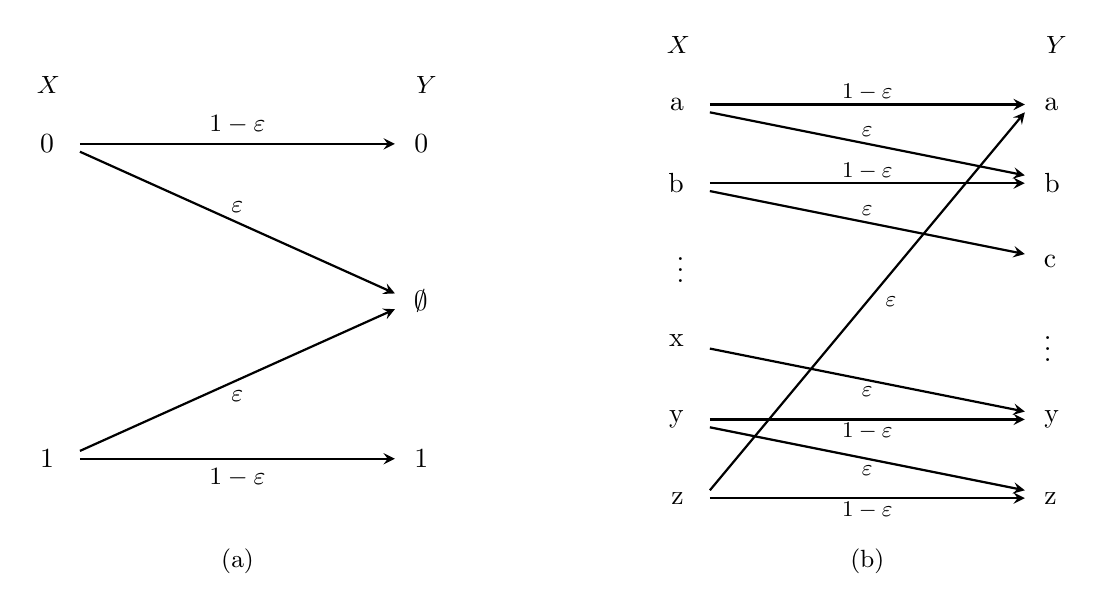
\begin{tikzpicture}
\shorthandoff{>}
%
% Canal borrador
\begin{scope}
\draw (-.4,2.75) node {\small $X$}; \draw (4.4,2.75) node {\small $Y$};
%
\draw[>=stealth,->,thick] (-.2,2) node[left]{0} (0,2) -- (4,2) node[right]{\ 0};
\draw (2,2) node[above]{\small $1-\varepsilon$};
%
\draw[>=stealth,->,thick] (-.2,-2) node[left]{1} (0,-2) -- (4,-2) node[right]{\ 1};
\draw (2,-2) node[below]{\small $1-\varepsilon$};
%
\draw[>=stealth,->,thick] (0,1.9)--(4,.1);
\draw (2,1.2) node{\small $\varepsilon$};
\draw[>=stealth,->,thick] (0,-1.9)--(4,-.1);
\draw (2,-1.2) node{\small $\varepsilon$};
\draw (4,0) node[right]{\ $\emptyset$};
%
\end{scope}
%
% Canal typewriter
\begin{scope}[xshift = 8cm]
\draw (-.4,3.25) node {\small $X$}; \draw (4.4,3.25) node {\small $Y$};
%
% lineas sin error
\draw[>=stealth,->,thick] (-.2,2.5) node[left]{a} (0,2.5) -- (4,2.5) node[right]{\ a};
\draw (2,2.65) node[scale=.9]{\small $1-\varepsilon$};
\draw[>=stealth,->,thick] (-.2,1.5) node[left]{b} (0,1.5) -- (4,1.5) node[right]{\ b};
\draw (2,1.65) node[scale=.9]{\small $1-\varepsilon$};
\draw (-.2,.5) node[left]{$\vdots$}; \draw (4,-.5) node[right]{\ $\vdots$};
\draw[>=stealth,->,thick] (-.2,-1.5) node[left]{y} (0,-1.5) -- (4,-1.5) node[right]{\ y};
\draw (2,-1.65) node[scale=.9]{\small $1-\varepsilon$};
\draw[>=stealth,->,thick] (-.2,-2.5) node[left]{z} (0,-2.5) -- (4,-2.5) node[right]{\ z};
\draw (2,-2.65) node[scale=.9]{\small $1-\varepsilon$};
%
% lineas con el error
\draw[>=stealth,->,thick] (0,2.4) -- (4,1.6);
\draw (2,2.15) node[scale=.9]{\small $\varepsilon$};
\draw[>=stealth,->,thick] (0,1.4) -- (4,.6); \draw (4,.5) node[right]{\ c};
\draw (2,1.15) node[scale=.9]{\small $\varepsilon$};
\draw[>=stealth,->,thick]  (-.2,-.5) node[left]{x} (0,-.6) -- (4,-1.4);
\draw (2,-1.15) node[scale=.9]{\small $\varepsilon$};
\draw[>=stealth,->,thick] (0,-1.6) -- (4,-2.4);
\draw (2,-2.15) node[scale=.9]{\small $\varepsilon$};
\draw[>=stealth,->,thick] (0,-2.4) -- (4,2.4);
\draw (2.3,0) node[scale=.9]{\small $\varepsilon$};
%
\end{scope}
\draw (2,-3.3) node{\small (a)};
\draw (10,-3.3) node{\small (b)};
\end{tikzpicture}
 \end{center}
%
\leyenda{Ejemplos de canales discretos usuales.  (a): canal borrador, donde un 0
  (de probabilidad de ocurrencia $r$) o 1 (de probabilidad de occurrencia $1-r$)
  puede  transmitirse correctamente or  ser borado/perdido  (estado $\emptyset$)
  con una  probabilidad $\varepsilon$.   Se calcula $I_2(X;Y)  = (1-\varepsilon)
  h_2(r)$, dando la capacidad $C_2  = 1-\varepsilon$, alcanzada para una entrada
  uniforme.   (b): canal tipo  machina de  escribir~\protect\footnotemark, donde
  cada letra  de un ensemble  de $n$  letras (ac\'a con  $n = 26$)  se transmite
  correctamente con una probabilidad $1-\varepsilon$  o a la letra siguiente (de
  manera c\'iclica) con una probabilidad $\varepsilon$.  De $I_n(X;Y) = H_n(Y) -
  H_n(Y|X) = H_n(Y)  - h_n(\varepsilon)$ se deduce que $I_n$  es m\'axima si $Y$
  es  uniforme,  lo que  es  posible  si  $X$ es  uniforma,  dando  $C_n =  1  -
  h_n(\varepsilon)$.}
\label{Fig:SZ:CanalesDiscretos}
\end{figure}
%
\footnotetext{Se mencionar\'a de  que en toda esta subsecci\'on,  no se necesita
  de que  $X$ y/o  $Y$ sean  variables aleatorias reales,  \ie pueden  tomar sus
  valores sobre cualquier espacio discreto (por ejemplo de letras).}


% ================================= canal gaussiano

\subseccion{Canal de transmisi\'on continuo gaussiano y su capacidad}
\label{Ssec:SZ:Canalgaussiano}

Un canal de  comunicaci\'on continuo relativamente simple es  conocido como {\it
  canal  gaussiano}~\cite[Sec.~25]{Sha48},~\cite{CovTho06,  Rio07}:  $X$ es  una
variable continua definida  sobre $\X \subseteq \Rset^d$ y la  salida $Y$ es una
versi\'on ruidosa de $X$, \ie $Y =  X + \xi$ con el ruido $\xi$ independiente de
$X$. En  el canal gaussiano, $\xi  \equiv \Gauss$ es un  vector gaussiano.  Este
canal es tambi\'en definido por  su densidad de probabilidad ``de transici\'on''
$p_{Y|X=x}(y)$,  \ie por  la distribuci\'on  del ruido.   Tal canal  es descrito
figura  Fig.~\ref{Fig:SZ:CanalGaussiano}.   Se  supone  conocida  la  matriz  de
covarianza $\Sigma_\Gauss$ del ruido, y se  nota $\Sigma_X$ la de la entrada. En
pr\'actica, no se puede mandar un mensaje a una potencia tan alta que se quiere,
lo que se traduce por una limitaci\'on
%
\[
\Tr\left(  \Sigma_X  \right) \le  \P,
\]
%
potencia l\'imite permitida por componente (sampleo).

\begin{figure}[h!]
%
\begin{center} 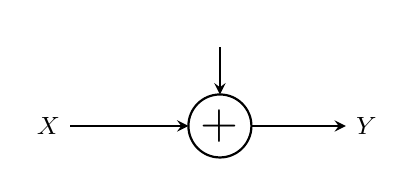
\begin{tikzpicture}
\shorthandoff{>}
%
%
% entrada
\draw[>=stealth,->,thick] (0,0) node[left]{\small $X$} --(1.5,0);
%
% adicion del ruido
\draw[thick] (1.9,0) circle (.4);
\draw[>=stealth,->,thick] (1.9,1) node[above]{\small $\N$} --(1.9,.4);
\draw (1.9,0) node[align=center,scale=1.5]{\large +};
%
% salida
\draw[>=stealth,->,thick] (2.3,0)--(3.5,0) node[right]{\small $Y$};
\end{tikzpicture}
 \end{center}
%
\leyenda{Canal gaussiano. La entrada $X$, modelizada por un vector aleatorio, es
  corrupta aditivamente por un ruido gaussiano $\Gauss$ independiente de $X$. La
  salida es entonces $Y = X + \Gauss$ y el canal es completamente descrito por \
  $p_{Y|X=x}(y)   =   p_{\Gauss}(y-x)$  \   (obviamente   independiente  de   la
  distribuci\'on de la entrada).}
%
\label{Fig:SZ:CanalGaussiano}
\end{figure}


Por  definici\'on, la informaci\'on  mutua $I(X;Y)$  entrada-salida es  dada por
$I(X;Y) = H(Y) - H(Y|X) = H(Y) - H(\Gauss)$. Maximizar $I(X;Y)$ es equivalente a
maximizar  $H(Y) =  H(X  + \Gauss)$  sujeto  a $\Tr\left(  \Sigma_X \right)  \le
\P$. Fijando  un $\Sigma_X$, la  propiedad~\ref{Prop:SZ:cotamaximagaussiana} \ de
la entrop\'ia diferencial implica que $H(Y)$  sea m\'axima si y solamente si $Y$
es gaussiana,  es decir  si y solamente  si $X$  est gaussiana, dando  $I(X;Y) =
\frac12  \log \left|  \Sigma_X +  \Sigma_\Gauss  \right| -  \frac12 \log  \left|
  \Sigma_\Gauss \right|$. Tomando en cuenta  el l\'imite de potencia, hace falta
maximizar $\left| \Sigma_X  + \Sigma_\Gauss \right|$ sujeto a  $\Tr \Sigma_X \le
\P$ \  y \ $\Sigma_X  \ge 0$ sim\'etica  lo que no  es trivial.  Se  encuentra el
enfoque  permitiendo solucionar  el problema  en~\cite[Sec.~9.4]{CovTho06}.  Sea
$U$, matriz  ortogonal ($U U^t =  U^t U = I$)  de los autovectores  de la matriz
$\Sigma_\Gauss  \ge 0$  sim\'etica~\footnote{Se  recordar\'a de  que  $A \ge  0$
  significa que $A$  es definida no negativa.}, de  columnas $u_i$ ordenadas tal
que los autovalores corespondientes  $\lambda^\Gauss_i$ sean en orden creciente,
\ie
%
\[
\Sigma_\Gauss  =  U \diag\left(  \lambda^\Gauss_1  ,  \ldots ,  \lambda^\Gauss_d
\right)  U^t \qquad  \mbox{con} \qquad  0  \le \lambda^\Gauss_1  \le \cdots  \le
\lambda^\Gauss_d,
\]
%
donde $\diag$ es la matriz diagonal teniendo los $\lambda_i$ en su diagonal. Sea
\  $R_X  =  U^t  \Sigma_X  U$.   Es  sencillo  ver  que  \  $\left|  \Sigma_X  +
  \Sigma_\Gauss \right|  = \left| R_X +  \Lambda_\Gauss \right|$ \ (de  $|A B| =
|A| \,  |B|$) \ y  que \ $\Tr \Sigma_X  = \Tr R_X$  (de $\Tr(A B) =  \Tr(B A)$).
Entonces,  el problema  se reduce  a maximizar  \ $\left|  R_X  + \Lambda_\Gauss
\right|$  \ sujeto  a \  $\Tr R_X  \le \P$  \ y  \ $R_X  \ge 0$  sim\'etica.  La
desigualdad de Hadamard ya evocada da \ $\left| R_X + \Lambda_\Gauss \right| \le
\prod_i \left(  R_X + \Lambda_\Gauss  \right)_{i,i} = \prod_i \left(  \left( R_X
  \right)_{i,i} +  \lambda^\Gauss_i \right)$  \ donde $(\cdot)_{i,i}$  denota la
componente $i,i$  de la  matriz, con  igualdad si y  solamente si  \ $R_X$  \ es
diagonal: para maximizar \ $\left| R_X + \Lambda_\Gauss \right|$, \ $R_X$ \ debe
ser diagonal (dada una diagonal, se  alcanza el m\'aximo si los otros t\'erminos
son  nulos).  Es  decir que  la base  que diagonaliza  \ $\Sigma_\Gauss$  \ debe
diagonalizar  tambi\'en  $\Sigma_X$.   Sean  \ $\lambda^X_i$  \  los  t\'erminos
diagonales  de  $R_X$: queda  que  maximizar  \  $\prod_i \left(  \lambda^X_i  +
  \lambda^\Gauss_i  \right)$  \ sujeto  a  $\sum_i \lambda^X_i  \le  \P$  \ y  \
$\lambda^X_i \ge 0$.   Este problema de optimizaci\'on sujeto  a una desigualdad
se  resuelva  con el  enfoque  de  Karush-Kuhn-Tucker~\footnote{Se introduce  el
  factor  de   Lagrange  y   se  maximiza  \   $\prod_i  \left(   \lambda^X_i  +
    \lambda^\Gauss_i \right) + \eta  \sum_i \lambda^X_i$.  Eso da \ $\lambda^X_i
  + \lambda^\Gauss_i = \lambda$ \ constante si $\lambda$ es tal que se satisfaga
  la positividad de $\lambda^X_i$, y  $\lambda^X_i = 0$ sino. En otras palabras,
  \ $\lambda^X_i = \left( \lambda - \lambda^\Gauss_i \right)_+$ con $\lambda$ el
  factor  de Lagrande  despu\'es de  una  reescritura. Queda  que maximizar  los
  $\lambda^X_i$ para  maximizar $\left| R_X + \Lambda_\Gauss  \right|$, es decir
  tomar  $\lambda$ lo  m\'as grande  que  se puede,  pero satisfaciendo  $\sum_i
  \lambda^X_i   \le  \P$,   \ie   alcanzando  la   igualdad.\label{Foot:SZ:KKT}}
(KKT)~\cite{Mil00,  CamMar09},   dando  \   $\lambda^X_i  =  \left(   \lambda  -
  \lambda^\Gauss_i  \right)_+$  \  con  \  $(\cdot)_+ =  \max(\cdot,0)$  \  y  \
$\lambda$ \ tal que \ $\sum_i \left( \lambda - \lambda^\Gauss_i \right)_+ = \P$.
En conclusi\'on, la capacidad es dada por
%
\begin{eqnarray*}
C =  \frac12 \log \left(  \frac{\left| \Sigma_\Gauss +  \Sigma_X \right|}{\left|
      \Sigma_\Gauss  \right|}  \right)  & \quad \mbox{con} \quad &  \Sigma_X  =  U
\diag\left( \left(\lambda - \lambda^\Gauss_1\right)_+ , \ldots , \left(\lambda -
    \lambda^\Gauss_d \right)_+ \right) U^t,\\[2.5mm]
%
& &  \lambda \ \mbox{ tal que } \:
\sum_i \left(\lambda - \lambda^\Gauss_i \right)_+ = \P
\end{eqnarray*}
%
alcanzada por $X$ gaussiano de matriz de covarianza $\Sigma_X$ as\'i construida.

La  \'ultima condici\'on  se resuelva  a  trav\'es de  lo que  es conocido  como
``llenado   de   agua''   (water-filling   en   ingl\'es),   illustrado   figura
Fig.~\ref{Fig:SZ:WaterFilling}.   El  principio  es  parecido  a  tener  niveles
$\lambda^\Gauss_i$  representando  las  potencias  del  ruido (en  la  base  que
diagonaliza la  matriz de covarianza), y  de ``llenar con agua''  hasta un nivel
$\lambda$ tal que el ``volumen''  a\~nadido vale $\P$; en cada $\lambda^\Gauss_i$
se ha a\~nadido el $\lambda^X_i$~\cite[Sec.~9.4]{CovTho06}.

\begin{figure}[h!]
%
\begin{center} \begin{tikzpicture}
\shorthandoff{>}
%
% Filling
\filldraw[fill=gray!30] (3,2)--(3,1.5)--(2,1.5)--(2,1)--(1,1)--(1,.75)--(0,.75)--(0,2);
%
%Axes
\draw[>=stealth,->] (-.1,0)--(6,0);% node[right]{\small $i$};
\draw[>=stealth,->] (0,-.1)--(0,3);
\draw (0,.85) node[left]{\rotatebox{90}{\footnotesize Potencias}};
%
% neveles de ruido
\draw[thick] (0,.75)--(1,.75)--(1,0); \draw(.5,.375) node{\small $\lambda^\N_1$};
\draw[thick] (1,.75)--(1,1)--(2,1)--(2,0); \draw(1.5,.5) node{\small $\lambda^\N_2$};
\draw[thick] (2,1)--(2,1.5)--(3,1.5)--(3,0); \draw(2.5,.75) node{\small $\lambda^\N_3$};
\draw[thick] (3,1.5)--(3,2.25)--(4,2.25)--(4,0); \draw(3.5,1.125) node{\small $\lambda^\N_4$};
\draw[thick] (4,2.25)--(4,2.75)--(5,2.75)--(5,0); \draw(4.5,1.375) node{\small $\lambda^\N_5$};
\draw[thick] (5.5,1.25) node{\bf $\cdots$};
%
% nivel lambda y potencias de los X
\draw[thick] (0,2) node[left]{\small $\lambda$}--(3,2);
\draw (1,.75)--(1,2); \draw (.5,1.375) node{\small $\lambda^X_1$};
\draw (2,1)--(2,2); \draw (1.5,1.5) node{\small $\lambda^X_2$};
\draw (3,1.5)--(3,2); \draw (2.5,1.75) node{\small $\lambda^X_3$};
\end{tikzpicture}
 \end{center}
%
\leyenda{Principio   del  ``water-filling''   para  obtener   los  $\lambda^X_i$
  satisfaciendo  el v\'inculo de  potencia l\'imite  y permitiendo  de construir
  $\Sigma_X$ a partir  de la matriz diagonal de los $\lambda^X_i$  y la base que
  diagonaliza  la  covarianza  $\Sigma_\Gauss$  del  ruido.  La  zona  en  grise
  representa esquem\'aticamente $\P$.}
%
\label{Fig:SZ:WaterFilling}
\end{figure}

En   el   caso   escalar,   se   obtiene
%
\[
C = \frac12 \log\left( 1 + \frac{\P}{\sigma_\Gauss^2} \right),
\]
%
donde     $\frac{\P}{\sigma_\Gauss^2}$     es     conocido    como     relaci\'on
se\~nale-ruido~\footnote{Esta formula es muy  parecida a la de Shannon, Laplume,
  o Clavier~\cite{Sha48,  Lap48, Cla48} (ver tambi\'en~\cite[Sec.~9.3]{CovTho06}
  o~\cite[Sec.~11.2]{Rio07}).   De hecho,  si se  considera  s\'imbolos mandados
  durante  $T$ segundos  cada  uno (s\'imbolos  puestos  en forma  para dar  una
  se\~nal anal\'ogica) usando una banda  de transmisi\'on $B$, por el teorema de
  Nyquist $B = \frac{1}{2 T}$ (caso l\'imite). Si el ruido es blanco en la banda
  $B$, de densidad espectral de potencia por unidad de frecuencia igual a $N_0$,
  para  un  s\'imbolo  la  relaci\'on  se\~nal-ruido  se  escribe  $\frac{\P}{N_0
    B}$. Adem\'as,  se calcula en general  la capacidad por unidad  de tiempo es
  decir la capacidad  por s\'imbolo divido por  $T = \frac{1}{2 B}$, \ie  $C = B
  \log\left( 1 +  \frac{\P}{N_0 B} \right)$ por segundos,  lo que es precisamente
  la capacidad calculdada por Shannon.  Esta es a veces conocida como formula de
  Shannon-Hartley.}

En~\cite{CovTho06,  Rio07}  por ejemplo,  se  dan  otros  ejemplos de  canal  de
comunicaci\'on   en   el   contexto   continuo   (entrada   $X_t$   siendo   una
se\~nal/proceso, canal filtrando, canal con retroacci\'on (o feedback), etc.).

% ================================= codificacion

\subseccion{Codificaci\'on entr\'opica sin perdida}
\label{Ssec:SZ:Codificacion}

El  problema  de  codificaci\'on  de  fuente  puede  presentarse  de  la  manera
siguiente~\cite[cap.~5]{CovTho06}  o   \cite[cap.~13]{Rio07}.   Sea  un  proceso
aleatorio $\left\{  X_t \right\}_{t \in \Zset}$,  supuesto estacionario, llamado
{\it  fuente}, donde  los $X_t$  toman sus  valores sobre  un  alfabeto discreto
finito no necesariamente real ($X$ puede tomar cualquier etiqueta)
%
\[
\X = \{ x_1 , \ldots , x_\alpha \} \qquad \mbox{alfabeto fuente},
\]
%
de  distribuci\'on  $p_X$.   A  cada posible  secuencia~\footnote{Por  abuso  de
  escritura una  cadena de  $n$ s\'imbolos puede  ser vista como  un $n$-uplet.}
$s_1  \cdots s_n \in  \X^n$ de  letras de  $\X$, se  quiere asignar  un c\'odigo
$c(s_1 \cdots s_n)$ de letras de un alfabeto discreto finito,
%
\[
\C = \{ \cod_1 , \ldots , \cod_d \} \qquad \mbox{ alfabeto c\'odigo}.
\]
%
El c\'odigo es dicho {\it $d$-ario}.   Por ejemplo, se puede asignar un c\'odigo
$c(x_i)  = \cod_{i,1}  \cdots  \cod_{i,l_i} \in  \C^{l_i}$  a cada  s\'imbolo $x_i$,
c\'odigo llamado  {\it palabras c\'odigos}, y  a secuencias $s_1  \cdots s_n$ la
concatenaci\'on de las palabras  c\'odigos correspondiente a cada s\'imbolo, \ie
el  c\'odigo $c(s_1) \cdots  c(s_n)$.  En  el sistema  Moorse por  ejemplo, $\C$
consiste en  un punto,  una barra,  una espacio entre  letras, un  espacio entre
palabras.  En una computadora en general todo  se codifica en bits $\C = \{ 0 \,
, \, 1\}$.  M\'as formalmente, sean
%
\[
F_\X   =   \bigcup_{k=0}^{\infty}   \X^k   \qquad   \mbox{y}   \qquad   F_\C   =
\bigcup_{k=0}^{\infty} \C^k,
\]
%
uni\'on  de  secuencias de  $k$  letras de  $\X$  y  $\C$ respectivamente.   Una
codificaci\'on  de fuente  consiste en  una funci\'on  de \  $F_\X$ \  dentro de
$F_\C$. En lo que sigue, nos concentramos en c\'odigos definidos para bloques de
s\'imbolos de tama\~no $m \ge 1$:
%
\[
\begin{array}{lccl}
c_m: & \X^m & \rightarrow & F_\C\\[.5mm]
%
& x & \mapsto & c_m(x) \in \C^{l_{c_m}(x)}
% &
\end{array},
\]
%
donde $l_{c_m}(x) \in \Nset^*$ es el  {\it largo} de la palabra c\'odigo $c_m(x)$,
y
%
\[
\forall \, n \ge 1, \quad \forall  \, s_1 \cdots s_n \in \X^{n m}, \quad c_m(s_1
\cdots s_n) \equiv c_m(s_1) \cdots c_m(s_n),
\]
%
lo  que  es  llamado {\it  extensi\'on  del  c\'odigo}.   En  lo que  sigue,  se
escribir\'a $c \equiv c_1$.

Una manera ingenua de codificar consiste a apoyarse sobre la descomposici\'on de
base \ $d$  \ de un entero, \ie para  $1 \le i \le \alpha$  se puede escribir de
manera \'unica \ $i-1 = (i_0-1) + (i_1-1) d + \cdots + (i_K-1) d^K$ \ donde \ $K
= \Big\lceil \log_d |\X| \Big\rceil$ \ y \ $1 \le i_k \le \alpha$.  Entonces, se
puede asignar la palabra c\'odigo \ $c(x_i) = \cod_{i_0} \cdots \cod_{i_k}$ \ al
s\'imbolo  $x_i$.  Haciendo  eso, cada  palabra c\'odigo  tieno el  mismo largo.
Pero, es m\'as  econ\'omico hacer una codificaci\'on dicha  de largos variables,
teniendo   en  cuenta  las   probabilidades  de   aparici\'on  de   cada  $x_i$.
Implicitamente, es la idea del c\'odigo  de Moorse, que asigna un punto o series
de puntos o  c\'odigo peque\~no a las letras muy frecuentes  (ej.  un punto para
el `e',  dos puntos para el  `i', etc.), y  barras o combinaciones largas  a las
letras que son raras (ej. bara-bara-punto-bara para el `q' o cinco baras para el
`0').  Dicho de  otra manera, el c\'odigo ingenuo  ser\'ia ``eficaz'' para $x_i$
apareciendo con las mismas frecuencias/probabilidades.

En los c\'odigos de largos variables (incluyendo el c\'odigo ingenuo), volviendo
a  $c_m$, existen  varios tipos  de  c\'odigos.  Un  c\'odigo es  dicho {\it  no
  singular} si $c_m$  es inyectiva: a cada $x \in  \X^m$ corresponde una palabra
c\'odigo \'unica. Esta propiedad es un requisito que parece obvio querer para un
c\'odigo.  Pero  no es suficiente  para poder decodificar un  mensaje, compuesta
por una  secuencia de palabras  c\'odigo.  Lo importante  en este caso  es poder
decodificar  la   secuencia  sin  ambig\"uedad:  un  c\'odigo   est  dicho  {\it
  descifrable} o {\it  a decodificaci\'on \'unica} (o sin  perdida) si todas las
extensiones son no singulares.
%
\begin{ejemplo}[C\'odigo no singular, pero no decifrable]
\label{Ej:SZ:CodigoNoSingularDecifrable}
%
  Sean, sean \ $\X = \{ \aleph \, ,  \, \beth \, , \, \gimel \, , \daleth \}$, \
  $\C = \{0 \, , \, 1 \}$ \ y \ $c(\aleph) = 0, \: c(\beth) = 00, \: c(\gimel) =
  1,  \: c(\daleth)  = 01$  ($m =  1$).   El c\'odigo  es no  singular, pero  no
  descifrable.       La     secuencia      $0010$     puede      provenir     de
  $\aleph\aleph\gimel\aleph$,   \  de   \   $\aleph\daleth\aleph$  \   o  de   \
  $\beth\gimel\aleph$.
\end{ejemplo}
%
Obviamente,  se  requiere  en  general  de  un  c\'odigo  que  sea  descifrable.
Frecuentemente,  se requiere tambi\'en  poder decodificar  sobre la  marcha, sin
esperar de medir toda la secuencia  codificada: es lo que se llama {\it c\'odigo
  instantaneo}.
%
\begin{ejemplo}[C\'odigo decifrable, pero no instantaneo]
\label{Ej:SZ:CodigoDcifrableNoInstantaneo}
%
  Sea el  c\'odigo $c(\aleph)  = 00,  \: c(\beth) =  10, \:  c(\gimel) =  11, \:
  c(\daleth)  =  110$.  Este  c\'odigo  es  descifrable,  pero  no  instantaneo.
  Considera la secuencia  $0011011$ y marcha sobre ella.  $0$  no es una palabra
  c\'odigo; $00$  es y sin  ambig\"uedad proviene de  un $\aleph$ (no  hay otras
  palabras  empezando por $00$);  luego $1$  no es  una palabra,  y $11$  es una
  palabra  c\'odigo,  pero se  necesita  adelantar para  saber  si  viene de  un
  $\gimel$ o de un $\daleth$; la  letra siguiente siendo un $0$, todav\'ia no se
  puede concluir si $110$ vino de  $\gimel$ y alg\'o o $\daleth$.  Al final, con
  $1101$, se  sabe que se tuvimos  un $\daleth$ porque  ninguna palabra c\'odigo
  empieza por $01$.   Al final, sin ambig\"uedad el  antecedente de la secuencia
  binaria era  $\aleph\daleth\gimel$.  Pero se necesit\'o marchar  sobre toda la
  secuencia antes de decodificar.
\end{ejemplo}
%
Obviamente,  un c\'odigo  instantaneo es  tal  que ninguna  palabra c\'odigo  es
prefijo de una otra, \ie si $c_m(x)$ es una palabra c\'odigo, las otras palabras
c\'odigo no  pueden empezar  con $c_m(x)$; el  c\'odigo es tambi\'en  dicho {\it
  libre  de  prefijo}.   Estas   distinciones  estan  ilustradas  en  la  figura
Fig.~\ref{Fig:SZ:ClasesCodigos} (ver~\cite[cap.~5]{CovTho06}).

\begin{figure}[h!]
%
\begin{center} 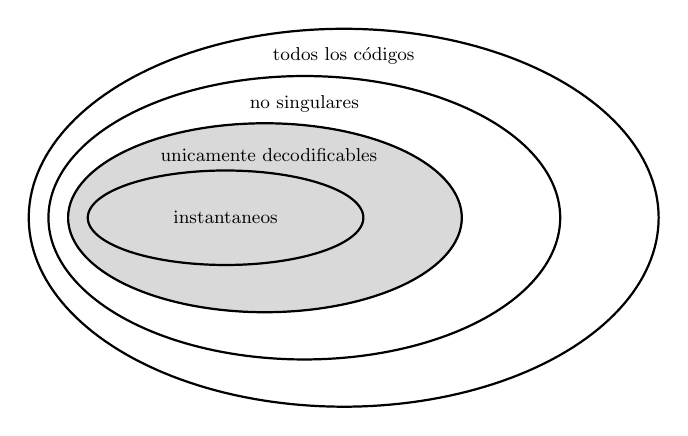
\begin{tikzpicture}
\shorthandoff{>}
\filldraw[fill=gray!30,domain=0:360, samples=200] plot ({2.5*cos(\x)+.5},{1.2*sin(\x)});
%%%%
\draw[thick,domain=0:360, samples=200] plot ({1.75*cos(\x)},{.6*sin(\x)});
\node[scale=.75] at (0,0){\small instantaneos};
%
\draw[thick,domain=0:360, samples=200] plot ({2.5*cos(\x)+.5},{1.2*sin(\x)});
\node[scale=.75] at (.55,.8){\small  unicamente decodificables};
%
\draw[thick,domain=0:360, samples=200] plot ({3.25*cos(\x)+1},{1.8*sin(\x)});
\node[scale=.75] at (1,1.45){\small no singulares};
%
\draw[thick,domain=0:360, samples=200] plot ({4*cos(\x)+1.5},{2.4*sin(\x)});
\node[scale=.75] at (1.5,2.05){\small todos los c\'odigos};
\end{tikzpicture}
 \end{center}
%
\leyenda{Clases  de c\'odigos.   Los  c\'odigos  contienen la  clase  de los  no
  singulares.  La misma  contiene la clase de los  c\'odigos descifrables.  Ella
  contiene los  c\'odigos instantaneos.  En  grise se representan las  clases de
  c\'odigos sin perdida a lo cuales se dedica esta secci\'on.}
%
\label{Fig:SZ:ClasesCodigos}
\end{figure}

Adem\'as  de   la  decodificaci\'on  sin   ambig\"uedad,  una  caracterizaci\'on
importante del  c\'odigo es la  taza de codificaci\'on~\footnote{En~\cite{Rio07}
  por  ejemplo, se  define esta  taza suponiendo  que cada  secuencia  fuente es
  codificada por el  mismo n\'umero de bits. La taza es  entonces el n\'umero de
  bits por s\'imbolo.}
%
\[
R_{c_m} = \frac{\log_d \left( \sum_{x \in \X^m} l(x) P(X = x) \right)}{m},
\]
%
donde $X$  representa una  secuencia de $m$  variables $X_t$.  El  argumento del
logaritmo (de base adecuada al cardinal  de $\C$) es el {\it largo promedio} del
c\'odigo. Por ejemplo,  para $d = 2$, $R_{c_m}$ es el  n\'umero de bits promedio
del c\'odigo por s\'imbolo.

En general,  se quiere minimizar $R_{c_m}$  (compresar el mensaje  a mandar), lo
que puede  ser contradictorio con la  necesidad de a\~nadir  redundancia para no
perder  informaci\'on   durante  una  transmisi\'on.   En  lo   que  sigue,  nos
concentramos en  el problema  de compresi\'on,  sin tener en  cuenta el  paso de
transmisi\'on  de  mensajes codificados  en  un  canal.   Minimizar la  taza  es
equivalente a minimizar el largo  promedio. Adem\'as, se puede focalisarse en $m
= 1$; todo se extiende sencillamente a $m > 1$.

La meta de  la compresi\'on es entonces construir  un c\'odigo $c$, descifrable,
que minimizar el largo promedio
%
\[
L(c) = \sum_{x \in \X} p_X(x) \, l(x).
\]
%
Antes de  ir m\'as adelante, hace  falta traducir en ecuaci\'on  el v\'inculo de
que   $c$   sea   descifrable.    Eso    es   dado   por   la   desigualdad   de
Kraft-McMillan~~\cite{Kra49,   McM56,   Kar61}~\footnote{Esta  desigualdad   fue
  probabada  por  L.  G.   Kraft  para c\'odigos  instantaneos  en  su tesis  de
  maestria~\cite{Kra49}.  Luego, fue extendida  a los c\'odigos descifrables por
  B.  McMillan~\cite{McM56} (en  una nota de pie de pagina  de su papel, atribua
  esta  observaci\'on a J.   L.  Doob  hecha oralemente  durante una  escuela de
  verano en Ann Arbor, MI en agosto 1955).}
%
\begin{teorema}[Desigualdad de Kraft-McMillan]
\label{Teo:SZ:KraftMcMillan}
%
  Los largos  $l_c(x)$ de las palabras  c\'odigo de un  c\'odigo $c$ descifrable
  deben satisfacer la desigualdad
  %
  \[
  \sum_{x \in \X} d^{-l_c(x)} \le 1.
  \]
  %
  Rec\'iprocamente,  para cada  conjunto de  enteros $\{  \ell_x \}_{x  \in \X}$
  satisfaciendo  esta   desigualdad,  es   posible  de  construir   un  c\'odigo
  descifrable con $l_c(x) = \ell_x$.
\end{teorema}
%
\begin{proof}
  Para cualquier $k \ge 1$ y cualquiera  cadena $s = s_1 \cdots s_k \in \X^k$, la
  extensi\'on  del  c\'odigo,  $c_k(s_1  \cdots  s_k) =  c(s_1)  \cdots  c(s_k)$
  satisface $l_{c_k}(s) = \sum_{i=1}^k l_c(s_i)$. Entonces
  %
  \[
  \left(  \sum_{x  \in \X}  d^{-l_c(x)}  \right)^k \:  =  \:  \sum_{\bar{x} \in  \X^k}
  d^{-l_{c_k}(\bar{x})} \: = \: \sum_{m=1}^{k \, l_c^{\max}} \#(m) \, d^{-m},
  \]
  %
  re-escribiendo  la segunda  suma, agrupando  los t\'erminos  de  mismo largos,
  donde $\#(m)$  es el n\'umero de c\'odicos  de $\X^k$ teniendo el  largo $m$ y
  $l_c^{\max}  =  \max_{x  \in  \X}  l_c(x)$  es el  largo  mayor.   $c$  siendo
  descifrable,  $c_k$ debe  ser inyectiva,  imponiendo $\#(m)  \le d^m$  (no hay
  m\'as palabras de  largo $m$ que el cardinal  de $\C^m$), dando inmediatemente
  que necesariamente
  %
  \[
  \forall \,  k \in \Nset^*, \quad \sum_{x  \in \X} d^{-l_c(x)} \le  \left( k \,
    l_c^{\max}  \right)^{\frac1k} \quad  \Leftrightarrow \quad  \sum_{x  \in \X}
  d^{-l_c(x)} \le \min_{k \in \Nset^*} \left( k \, l_c^{\max} \right)^{\frac1k}.
  \]
  %
  Un estudio r\'apido de \  $u \mapsto \left( u \, l_c^{\max} \right)^{\frac1u}$
  \ para \  $u \ge 1$ \ y  teniendo en cuenta de que $l_c^{\max}  \le 1$ permite
  concluir  que el  m\'inimo  es igual  a  1, terminando  la  parte directa  del
  teorema.

  Rec\'iprocamente, sea  \ $\{ \ell_x  \}_{x \in \X}$  \ un conjunto  de enteros
  satisfaciendo la  desigualdad de Kraft-McMillan.  Se puede  agrupar los largos
  iguales y  clasificarlos. Sea \ $n_\ell$ \  los n\'umeros de largos  igual a \
  $\ell =  1 , \ldots  , \ell^{\max} \le  \alpha$.  Consideramos ahora  un arbol
  empezando con una ra\'iz, correspondiente a un largo $0$, que se divide en $d$
  ramas, correspondiente a los largos iguales  a $1$; a cada nudo se asocian las
  letras \  $\cod_1, \ldots , \cod_d$. Esto  nudos se dividen cada  uno en $d$
  otras  ramas, y  los nudos  de ``padre''  \ $\cod_i$  \ se  va a  asociar las
  palabras c\'odigos \ $\cod_i \cod_1 , \ldots , \cod_i \cod_\alpha$, \ etc.
  Este  arbol,  conocido  como  arbol  de  Kraft,  es  ilustrado  en  la  figura
  Fig.~\ref{Fig:SZ:ArbolKraft}  para \  $d =  2$  \ y  \ $\C  =  \{0 \,  , \,  1
  \}$. Claramente, \ $n_1 \le d$ \ si no \ $n_1 \, d^{-1} > 1$ \ y los largos no
  podr\'ian  satisfacer  la  desigualdad  de Kraft-McMillan.   El  principio  es
  entonce de asociar a los \ $n_1$ \ (posiblemente igual a 0) largos iguales a \
  $1$ \ unos nudos con las palabras c\'odigo asociadas de largo \ $1$ \ (primera
  profundez  de  ramas)  y de  prohibir  todos  las  ramas  de padre  los  nudos
  seleccionados        (lineas        punteadas        en       la        figura
  Fig.~\ref{Fig:SZ:ArbolKraft}). Estos  nudos son  llamados {\em hojas}  (no hay
  ramas).  En  la capa de ``hijos'' de  profundez/largos \ $2$, quedan  \ $d^2 -
  n_1 \, d$ \ nudos (accessibles)  que se pueden dividir en ramas.  Nuevamente, \
  $n_2 \le d^2 - n_1 \, d$ \  sino tendr\'iamos \ $n_1 \, d^{-1} + n_2 \, d^{-2}
  > 1$, \ incompatible con la  desigualdad de Kraft-McMillan. Se puede asociar a
  los \ $n_2$  \ largos iguales a \  $2$ \ unos nudos con  las palabras c\'odigo
  asociadas de  largo \ $2$  \ (segunda profundez),  y de prohibir que  salen de
  estos nudos  nuevas ramas (son entonces  hojas en la  segunda profundez), etc.
  Haciendo as\'i, se asocia un c\'odigo \  $c$ \ de largos \ $l_c(x) = \ell_x$ \
  que aparece libre  de prefijo, es decir instantaneo.   Entonces, este c\'odigo
  es tambi\'en descifrable.
\end{proof}

A este punto, se menciona los hechos siguientes
%
\begin{itemize}
\item  Los  largos de  un  c\'odigo  descifrable  satisfacen la  desigualdad  de
  Kraft-McMillan,  pero con  el  conjunto de  largos  correspondientes se  puede
  siempre  construir un c\'odigo  instantaneo.  Claramente,  se puede  buscar un
  c\'odigo de largo promedio m\'inimo  en los c\'odigos instantaneo, sin perdida
  de optimalidad (buscar en la clase  m\'as amplia de los descifrable no permite
  bajar el largo promedio).
%
\item En  los c\'odigos  libres de prefijo,  si se  fija el n\'umero  de hojas
  (\'ultima   profundez)  borradas   contruyendo  un   c\'odigo,  este   vale  \
  $\sum_{i=1}^{\ell^{\max}}  n_i  \,  d^{\ell^{\max}  -  i} =  \sum_{x  \in  \X}
  d^{\ell^{\max} -  l_c(x)}$.  \ Es  necesariamente menor que el  n\'umero total
  $d^{\ell^{\max}}$  de hojas,  lo  que  prueba el  teorema  para los  c\'odigos
  instantaneos~\cite{Kra49, Kar61}.
%
\item El teorema  se generaliza obviamente para codificar  una fuente (discreta)
  con un n\'umero infinito de estados, tomando el l\'imite $\alpha \to \infty$.
%
\item Si se conocen los largos  \'optimos, es suficiente para poder construir un
  c\'odigo libre de prefijo.
\end{itemize}

\begin{figure}[h!]
%
\begin{center} 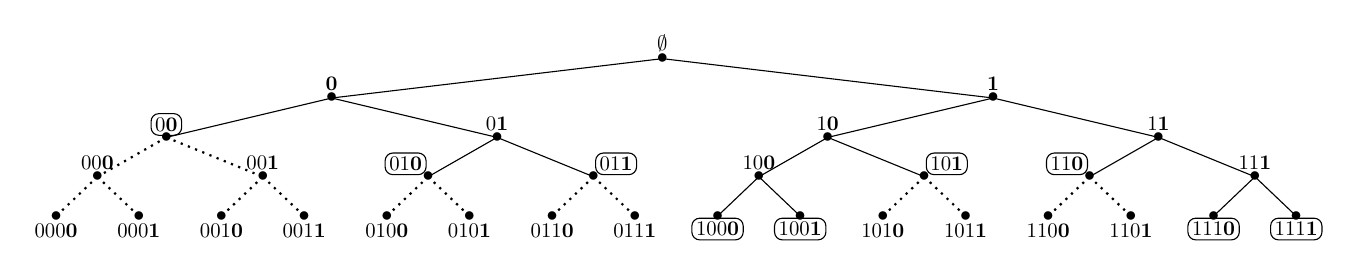
\begin{tikzpicture}[xscale=1.4]
\shorthandoff{>}
%
% nivel 2^4
%%%%%%%%%%%%
\draw[thick,dotted] (.375,.5)--(0,0) node[scale=.8]{$\bullet$} node[below,scale=.75]{000\textbf{0}};
\draw[thick,dotted] (.375,.5)--(.75,0) node[scale=.8]{$\bullet$} node[below,scale=.75]{000\textbf{1}};
\draw[thick,dotted] (1.875,.5)--(1.5,0) node[scale=.8]{$\bullet$} node[below,scale=.75]{001\textbf{0}};
\draw[thick,dotted] (1.875,.5)--(2.25,0) node[scale=.8]{$\bullet$} node[below,scale=.75]{001\textbf{1}};
\draw[thick,dotted] (3.375,.5)--(3,0) node[scale=.8]{$\bullet$} node[below,scale=.75]{010\textbf{0}};
\draw[thick,dotted] (3.375,.5)--(3.75,0) node[scale=.8]{$\bullet$} node[below,scale=.75]{010\textbf{1}};
\draw[thick,dotted] (4.875,.5)--(4.5,0) node[scale=.8]{$\bullet$} node[below,scale=.75]{011\textbf{0}};
\draw[thick,dotted] (4.875,.5)--(5.25,0) node[scale=.8]{$\bullet$} node[below,scale=.75]{011\textbf{1}};
%
\draw (6.375,.5)--(6,0) node[scale=.8]{$\bullet$}
node[inner sep=2pt,outer sep=1pt,draw=black,below,scale=.75,rounded corners=1mm]{100\textbf{0}};
%
\draw (6.375,.5)--(6.75,0) node[scale=.8]{$\bullet$}
node[inner sep=2pt,outer sep=1pt,draw=black,below,scale=.75,rounded corners=1mm]{100\textbf{1}};
%
\draw[thick,dotted] (7.875,.5)--(7.5,0) node[scale=.8]{$\bullet$} node[below,scale=.75]{101\textbf{0}};
\draw[thick,dotted] (7.875,.5)--(8.25,0) node[scale=.8]{$\bullet$} node[below,scale=.75]{101\textbf{1}};
\draw[thick,dotted] (9.375,.5)--(9,0) node[scale=.8]{$\bullet$} node[below,scale=.75]{110\textbf{0}};
\draw[thick,dotted] (9.375,.5)--(9.75,0) node[scale=.8]{$\bullet$} node[below,scale=.75]{110\textbf{1}};
%
\draw (10.875,.5)--(10.5,0) node[scale=.8]{$\bullet$}
node[inner sep=2pt,outer sep=1pt,draw=black,below,scale=.75,rounded corners=1mm]{111\textbf{0}};
%
\draw (10.875,.5)--(11.25,0) node[scale=.8]{$\bullet$}
node[inner sep=2pt,outer sep=1pt,draw=black,below,scale=.75,rounded corners=1mm]{111\textbf{1}};
%
%----------
%
% nivel 2^3
%%%%%%%%%%%%
\draw[thick,dotted] (1,1)--(.375,.5) node[scale=.8]{$\bullet$} node[above,scale=.75]{00\textbf{0}};
\draw[thick,dotted] (1,1)--(1.875,.5) node[scale=.8]{$\bullet$} node[above,scale=.75]{00\textbf{1}};
%
\draw (4,1)--(3.375,.5) node[scale=.8]{$\bullet$}
node[inner sep=2pt,outer sep=1pt,draw=black,above left,scale=.75,rounded corners=1mm]{01\textbf{0}};
%
\draw (4,1)--(4.875,.5) node[scale=.8]{$\bullet$}
node[inner sep=2pt,outer sep=1pt,draw=black,above right,scale=.75,rounded corners=1mm]{01\textbf{1}};
%
\draw (7,1)--(6.375,.5) node[scale=.8]{$\bullet$} node[above,scale=.75]{10\textbf{0}};
%
\draw (7,1)--(7.875,.5) node[scale=.8]{$\bullet$}
node[inner sep=2pt,outer sep=1pt,draw=black,above right,scale=.75,rounded corners=1mm]{10\textbf{1}};
%
\draw (10,1)--(9.375,.5) node[scale=.8]{$\bullet$}
node[inner sep=2pt,outer sep=1pt,draw=black,above left,scale=.75,rounded corners=1mm]{11\textbf{0}};
%
\draw (10,1)--(10.875,.5) node[scale=.8]{$\bullet$} node[above,scale=.75]{11\textbf{1}};
%
%----------
%
% nivel 2^2
%%%%%%%%%%%%
\draw (2.5,1.5)--(1,1) node[scale=.8]{$\bullet$}
node[inner sep=2pt,outer sep=1pt,draw=black,above,scale=.75,rounded corners=1mm]{0\textbf{0}};
%
\draw (2.5,1.5)--(4,1) node[scale=.8]{$\bullet$} node[above,scale=.75]{0\textbf{1}};
\draw (8.5,1.5)--(7,1) node[scale=.8]{$\bullet$} node[above,scale=.75]{1\textbf{0}};
\draw (8.5,1.5)--(10,1) node[scale=.8]{$\bullet$} node[above,scale=.75]{1\textbf{1}};
%
%----------
%
% nivel 2^1
%%%%%%%%%%%%
\draw (5.5,2)--(2.5,1.5) node[scale=.8]{$\bullet$} node[above,scale=.75]{\textbf{0}};
\draw (5.5,2)--(8.5,1.5) node[scale=.8]{$\bullet$} node[above,scale=.75]{\textbf{1}};
%
%----------
%
% nivel 2^0
%%%%%%%%%%%%
\draw (5.5,2) node[scale=.8]{$\bullet$} node[above,scale=.75]{$\emptyset$};

\end{tikzpicture} \end{center}
%
\leyenda{Arbol de  Kraft en el  caso binario ($d  = 2$). La ra\'iz,  de c\'odigo
  $\emptyset$ de largo 0, se divide en dos ramas, de c\'odigos respectivamente \
  $0$ \ y  \ $1$ \ (profundez \  $1$). Cada nudo de esta profundez  se divide en
  dos ramas (profundez dos), dando cuatros nuevos nudos con los c\'odigos \ $00$
  \ y $01$ de padre \ $0$, y \ $10$ \ y $11$ de padre \ $1$.  Etc.  En cada nudo
  de esta figura,  en el c\'odigo, se marca en  negrita la letra correspondiente
  al bit a\~nadido al c\'odigo padre.   Para hacer un c\'odigo libre de prefijo,
  una vez que un nudo es  seleccionado para ser una palabra c\'odigo (encuadrado
  en la  figura), no  puede tener nudos  ``hijos'' siendo tambi\'en  una palabra
  c\'odigo:  se boran  las ramas  saliendo  de un  nudo-palabra c\'odigo  (ramas
  punteadas).}
%
\label{Fig:SZ:ArbolKraft}
\end{figure}

El formalismo dado,  se va a ver ahora reaparecer la  entrop\'ia de Shannon como
cota de la codificaci\'on de fuente sin perdida:

\begin{teorema}[Cota inferior de c\'odigos descifrables]
\label{Teo:SZ:CotaInferiorCodigosDescifrables}
%
  Para  cualquier c\'odigo  \  $c$ \  descifrable  de la  fuente  $X$, su  largo
  promedio es  acotado por debajo  por la entrop\'ia  de Shannon de base  $d$ de
  $X$,
  %
  \[
  L(c) = \sum_{x \in \X} p_X(x) \, l_c(x) \: \ge \: H_d(X).
  \]
\end{teorema}
%
\begin{proof}
  Sea \ $q(x)  = \frac{d^{-l_c(x)}}{\sum_{x \in \X} d^{-l_c(x)}}$,  \ siendo una
  distribuci\'on de  probabilidad por  construcci\'on.  Escribiendo \  $l_c(x) =
  \log_d d^{-l_c(x)}$, \ se puede expresar el largo promedio de la forma
  %
  \[
  L(c) =  - \sum_{x  \in \X}  p_X(x) \, \log_d  d^{-l_c(x)} =  - \sum_{x  \in \X}
  p_X(x) \, \log_d q(x) - \log_d \sum_{x \in \X} d^{-l_c(x)}.
  \]
  %
  Notando que \ $- \log_d q  = \log_d \left( \frac{p_X}{q} \right) - \log_d p_X$
  \ se obtiene
  %
  \[
  L(c)  = H_d(X)  + D_{\mathrm{kl},d}\left(  \left.   p_X \right\|  q \right)  -
  \log_d \sum_{x \in \X} d^{-l_c(x)}.
  \]
  %
  El resultado proviene de la  positividad de la divergencia de Kullback-Leibler
  y de la desigualdad de Kraft-McMillan (el argumento del logaritmo siende menor
  que $1$).
\end{proof}
%
\noindent Este  resultado significa que la  taza de compresi\'on  sin perdida no
puede  ser m\'as  bajo que  el  contenido informacional  de la  fuente. En  este
sentido, $H$ tiene realmente un sabor de informaci\'on sobre la fuente $X$.

La entrop\'ia aparece tambi\'en en la cota superior del c\'odigo \'optimo:
%
\begin{teorema}[Cota superior del c\'odigo descifrable \'optimo]
\label{Teo:SZ:CotaSuperiorCodigoDescifrableOptimo}
%
  El largo promedio \ $L^\opt$ \ del c\'odigo \ $c^\opt$ \ descifrable, de largo
  promedio m\'inimo es  acotado por arriba por la entrop\'ia  de Shannon de base
  $d$ de $X$ m\'as un {\it dit} (1 s\'imbolo de $\C$),
  %
  \[
  L^\opt \: < \: H_d(X) + 1.
  \]
\end{teorema}
%
\begin{proof}
  Por  eso,  empezamos  por  buscar  los  largos  \'optimos,  soluci\'on  de  la
  optimizaci\'on
  %
  \[
  \min \sum_{x \in \X} p_X(x) \,  l(x) \qquad \mbox{sujeto a} \qquad \sum_{x \in
    \X} d^{-l(x)} \, \le \, 1.
  \]
  %
  %Sea \ $q(x)  = \frac{d^{-l_c(x)}}{\sum_{x \in \X} d^{-l_c(x)}}$,  \ siendo una
  %distribuci\'on de  probabilidad por  construcci\'on.  
  Escribiendo  \ $l_c(x) =  \log_d d^{-l_c(x)}$,  \ se  puede expresar  el largo
  promedio de la forma
  %
  \[
  L(c) =  - \sum_{x  \in \X}  p_X(x) \, \log_d  d^{-l_c(x)} =  - \sum_{x  \in \X}
  p_X(x) \, \log_d q(x) - \log_d \sum_{x \in \X} d^{-l_c(x)}.
  \]
  %
  Olvidando que los  \ $l_i \equiv l_c(x_i)$ \ son enteros,  $L(c)$ es convexa con
  respecto  a los $l_i$  as\'i que  el v\'inculo,  garantizando que  el m\'inimo
  existe y es \'unico.  El problema se resuelva con el enfoque KKT~\footnote{Ver
    nota de pie~\ref{Foot:SZ:KKT} pagina~\pageref{Foot:SZ:KKT}.}, optimizaci\'on
  con  v\'inculos tipo desigualdades~\cite{Mil00,  CamMar09}, conduciendo  a los
  ``largos''
  %
  \[
  \widetilde{l}(x) = - \log_d p_X(x).
  \]
  %
  $\widetilde{l}(x)$ no es necesariamente entero, as\'i que una posibilidad para
  volver  a largos  enteros  puede ser  de  tomar la  parte  entera superior  de
  $\widetilde{l}(x)$,
  %
  \[
  l(x) = \Big\lceil\! - \log_d p_X(x) \Big\rceil.
  \]
  %
  Obviamente el  conjunto de largos satisface la  desigualdad de Kraft-McMillan,
  as\'i que  se puede construir un  c\'odigo \ $c^\sh$ \  descrifrable con estos
  largos. De \ $l(x) < - \log_d p_X(x) + 1$ se obtiene
  %
  \[
   L^\opt \le L\left( c^\sh \right) < H_d(X) + 1.
  \]
  %
\end{proof}
%
De \[  H_d(X) \le  L^\opt < H_d(X)  + 1 \]  se revela  el rol fundamental  de la
entrop\'ia en la  codificaci\'on de fuente sin perdida.   La codificaci\'on es a
veces  dicha {\it  codificaci\'on  entr\'opica} y  da  un rol  operacional a  la
entrop\'ia  de  Shannon.   Se   notar\'a  tambi\'en  que  de  la  demostraci\'on
precediente  de   que  aparece  un   c\'odigo  particular  a  trav\'es   de  los
$\Big\lceil\!  - \log_d p_X(x) \Big\rceil$:
%
\begin{definicion}[C\'odigo de Shannon]
\label{Def:SZ:ShannonCode}
%
  Un  c\'odigo  \  $c^\sh$  \  de  una  fuente $X$,  de  largos  \  $l^\sh(x)  =
  \Big\lceil\!   - \log_d  p_X(x) \Big\rceil$,  \ libre  de  prefijo (construido
  sobre el arbol de Kraft) es llamado {\it c\'odigo de Shannon}.
\end{definicion}
%
Obviamente, tambi\'en
%
\[
H_d(X) \le L\left( c^\sh  \right) < H_d(X) +  1.
\]
%
Al lo contrario de primer vista, un  c\'odigo de Shannon no es \'optimo, como se
lo puede ver con el ejemplo siguiente.
%
\begin{ejemplo}
\label{Ej:SZ:CodigoShannonNoOpt}
%
  Sea \ $\X  = \C = \{ 0 \,  , \, 1 \}$ \  y una fuente $X$ tal que  \ $p_X(0) =
  0.999 = 1 - p_X(1)$.   Los largos de Shannon van a ser \ $l^\sh(0)  = 1$ \ y \
  $l^\sh(1) = 10$,  y el largo promedio vale \ $L\left(  c^\sh \right) = 1.009$.
  Obviamente, un c\'odigo \'optimo es \ $c(x) =  x$ \ de largos \ $l_c(x) = 1$ \
  dando \ $L^\opt = 1$ bit.
\end{ejemplo}
%
De hecho, volviendo al problema  con largos virtualmente no enteros, el m\'inimo
se alcanza para  $\widetilde{l}(x) = - \log_d p_X(x)$, es  decir que, los largos
siendo enteros, se alcanza la cota m\'inima del c\'odigo \'optimo si y solamente
si $- \log_d p_X(x)$.  Una distribuci\'on satifaciendo esta condici\'on es dicha
$d$-\'adica.   Sin embargo,  el c\'odigo  de  Shannon es  ``competitivo'' en  el
sentido de que:
%
\begin{teorema}[Competitividad del c\'odigo de Shannon]
\label{Teo:SZ:CompetitividadCodigoShannon}
%
  Sea $X$  \ fuente sobre  \ $\X$, de  distribuci\'on \ $p_X$  \ y \  $c^\sh$ el
  c\'odigo de Shannon asociado sobre el  alfabeto c\'odigo \ $\C = \{ \cod_1 ,
  \ldots  , \cod_d \}$,  de largos  $l^\sh(x) =  \Big\lceil\!  -  \log_d p_X(x)
  \Big\rceil$.  Para cualquier  c\'odigo \ $c$ \ descifrable  y cualquier $k \ge
  1$,
  %
  \[
  P\Big( l^\sh(X) \ge l_c(X) + k \Big) \le \frac{1}{d^{k-1}}.
  \]
\end{teorema}
%
\begin{proof}
  Por definici\'on de la parte entera superior, $a + 1 > \lceil a \rceil$, as\'i
  que $\lceil a \rceil \ge b \: \Rightarrow \: a > b-1$. A continuaci\'on, de la
  implicaci\'on de eventos $(Y  \ge a) \subset (Y \ge b-1)$ \  dando $P(A \ge a)
  \le P(Y \ge b-1)$ \ y de la definici\'on de un c\'odigo de Shannon se obtiene
  %
  \begin{eqnarray*}
  P\Big( l^\sh(X)  \ge l_c(X) + k  \Big) & \le & P\Big(  - \log_d p_X(X)
  \ge  l_c(X) + k  - 1  \Big)\\[2.5mm]
  %
  & = &  P\Big( p_X(X)  \le d^{-l_c(X)  - k  + 1} \Big)\\[2.5mm]
  %
  & = &  \sum_{x \in \X : p_X(x) \le d^{-l_c(x)  - k  + 1}} p_X(x)
  \end{eqnarray*}
  %
  Pero, sumando sobre  lo $x$ tal que $p_X(x) \le d^{-l_c(x)  - k + 1}$,
  se obtiene
  %
  \[
  %  \begin{eqnarray*}
  P\Big( l^\sh(X)  \ge l_c(X) + k  \Big) \le \frac{1}{d^{k-1}} \sum_{x  \in \X :
    p_X(x) \le d^{-l_c(x) - k + 1}} d^{-l_c(x)}
  %\\[2.5mm]
  %
  %P\Big( l^\sh(X) \ge l_c(X) + k \Big) & \le & 
  \le \frac{1}{d^{k-1}} \sum_{x \in \X} d^{-l_c(x)}
  \]
  %\end{eqnarray*}
  %
  (a\~nadiendo t\'erminos positivos en la suma). La prueba se cierra notando que
  $c$ siendo descifrable, $l_c$ satisface la desigualdad de Kraft-McMillan.
\end{proof}
%
Este teorema  traduce el hecho de  que a pesar  de que $c^\sh$ no  sea \'optimo,
tomando  cualquier otro c\'odigo,  incluyendo el  \'optimo, la  probabilidad que
$c^\sh(X)$ tenga un largo m\'as grande que $c(X)+k$ decrece exponencialmente con
$k$.
%
\begin{ejemplo}
\label{Ej:SZ:CompetitividadCodigoShannon}
%
  De manera general, con $d = 2$ y para $k = 9$, $P\Big( l^\sh(X) \ge l_c(X) + 9
  \Big)      \le       0.391      \%$.      En       particular,      en      el
  ejemplo~\ref{Ej:SZ:CodigoShannonNoOpt},    notando    que    s\'olo   en    la
  codificaci\'on de $x=1$ se puede tener $l^\sh(x) \ge l_c(x) + 9$, si no se usa
  1 bit, este resultado significa que la probabilidad de usar m\'as de 1 bit con
  el c\'odigo de Shannon es menor que $0.391 \%$. De hecho, una palabra c\'odigo
  de largo $10$ aparece con una probabilidad $0.1\%$\ldots
\end{ejemplo}

En el problema  de minimizaci\'on, el hecho de que los  largos deben ser enteros
no  permite  solucionar explicitamente  el  problema  de  busqueda del  c\'odigo
\'optimo.  N\'umeros investigadores  contruyeron c\'odigos, intentando probar de
que  eran \'optimos  (ver ej.~\cite{Sha48,  ShaWea64, Fan49}  por  los primeros,
y~\cite[\&  ref.]{CovTho06}).   El  c\'odigo  conocido  como  {\it  c\'odigo  de
  Fano}~\footnote{A pesar  de que sea  diferente del de  Shannon y que  cada uno
  fueron  hechos  independientemente,  a  veces  es conocido  como  c\'odigo  de
  Fano-Shannon, o aun Shannon-Fano-Elias~\cite{CovTho06, KraLiu15}.} \ $c^\fa$ \
se  basa  sobre  el  hecho  de   que  se  alcanza  la  cota  m\'inima  para  una
distribuci\'on $d$-\'adica.
%
\begin{definicion}[C\'odigo de Fano]
\label{Def:SZ:FanoCode}
%
  El  principio  es  de  clasificar   los  estados  de  $\X$  para  obtener  las
  probabilidades clasificadas en  orden decreciences ($p_X^\downarrow$).  Luego,
  se divide $\X$ en $d$ ensembles a  lo m\'as equiprobables que se puede (\ie de
  probabilidad a lo  m\'as cerca de $d^{-1}$) y de  asignar $\cod_i$ al conjunto
  $i$.   Luego,   se  repite  el   proceso  a  cada  sub-conjunto   (para  tener
  sub-conjuntos de probabilidades a lo m\'as cerca de $d^{-2}$) y al subconjunto
  $j$ del conjunto $i$ se va a asignar le c\'odigo $\cod_i \cod_j$, etc.  Eso es
  ilustrado en la figura Fig.~\ref{Fig:SZ:FanoHuffmanCodes}-(a).
\end{definicion}
%
\SZ{Probar/mencionar  que  tambi\'en  \[   H(X)  \le  L\left(  c^\fa  \right)  <
  H(X)+1. \]}
%  \qquad \mbox{con}  \qquad L^\fa  =  L_{c^\fa}$$}

Fijense de que no hay un \'unico c\'odigo  de Fano o de Shannon (tal como no hay
un \'optimo  \'unico).  Por exemple, hacer  una permutacion de  los $\cod_i$ da
los mismos  largos y  el mismo largo  promedio sin  cambiar el aspecto  libre de
prefijo. De la  misma manera, en el  arbol de Kraft, en cada  profundez se puede
permutar los s\'imbolos  asociados a las hojas de esta  profundez sin cambiar el
aspecto libre de  prefijo y sin que cambien los largos  $l(x_i)$ (y entonces con
el mismo largo promedio).

Una soluci\'on para construir un  c\'odigo \'optima fue propuesta por Huffman en
1951-1952~\cite{Huf52,  Pig03}~\footnote{De hecho,  Huffman  fue estudiantes  de
  maestria  de Fano,  trabajando  en el  MIT.  Su  tesis  era de  probar que  el
  c\'odigo de Fano  era \'optimo: Huffman propus\'o su  propio c\'odigo, andando
  al rev\'es del enfoque de Fano, y demostr\'o que era \'optimo~\cite{Sti91}.}
%
\begin{definicion}[C\'odigo de Huffman]
\label{Def:SZ:HuffmanCode}
%
  Suponemos que  existe un $\beta \in  \Nset$ tal que~\footnote{Si  no, se puede
    elegir $\beta =  \left\lceil \frac{\alpha-d}{d-1} \right\rceil$, y completar
    $\X$  con  $d  +  \beta  (d-1)  -  \alpha$  s\'imbolos  fuente  fictivos  de
    probabilidades ceros, lo  que no va a cambiar ni la  entrop\'ia, ni el largo
    promedio del  c\'odico aferente.}   $\alpha =  |\X| = d  + \beta  (d-1)$. El
  algoritmo de Huffman consiste a construir un arbol donde cada nudo es asociado
  a un conjunto de s\'imbolos fuente y una letra de $\C$ de la manera siguiente:
  %
  \begin{enumerate}
  \item\label{Huffman:clasificar}   Clasificar  las   probabilidades   en  orden
    decrecientes: por cambio de escritura, llamamos \ $p_i$ \ las probabilidades
    rearregladas y \ $x_i$ \ los s\'imbolo fuente correspondientes.
  %
  \item\label{Huffman:codigolocal}  A  cada \  $x_i,  \:  \alpha-d+1  \le i  \le
    \alpha$, \ associar un nudo y la letra ``hijo'' \ $\cod_i$.
  %
  \item\label{Huffman:padre} Crear \ $d$ \ ramas saliendo de un nudo padre hasta
    los $d$ nudos $x_i, \: \alpha-d+1 \le i \le \alpha$.
  %
  \item\label{Huffman:reconfiguracion}  Crear un  nuevo  conjunto de  s\'imbolos
    fuente  \  $\widetilde{x}_i   =  x_i,  \:  1  \le  i   \le  \alpha-d$  \  de
    probabilidades   respectivas    \   $\widetilde{p}_i   =   p_i$    \   y   \
    $\widetilde{x}_{\alpha-d+1} = \{  x_j, \: \alpha-d+1 \le j  \le \alpha$ \ de
    probabilidad  \  $\widetilde{p}_{\alpha-d+1}  =  p_{\alpha-d+1} +  \ldots  +
    p_\alpha$.  El \'utimo ``super-s\'imbolo''  fuente es asociado al nudo padre
    de la etapa~\ref{Huffman:padre}.
  %
  \item  Si   quedan  m\'as  de   un  (super-)s\'imbolo  fuente,  volver   a  la
    etapa~\ref{Huffman:clasificar}  con \  $p  \equiv \widetilde{p}$  \  y \  $x
    \equiv \widetilde{x}$.
  \end{enumerate}
  %
  Como descrito tratando del c\'odigo  usando el arbol de Kraft, \ $c^\huf(x_i)$
  \ se construye saliendo de la ra\'iz del arbol as\'i construido, agregando las
  letras del camino que  llega hasta la hoja \ $x_i$.  \  Eso es ilustrado en la
  figura Fig.~\ref{Fig:SZ:FanoHuffmanCodes}-(b) en el caso binario.
\end{definicion}
%
Se mencionar\'a que  a cada etapa, el nuevo  conjunto de super-s\'imbolos fuente
contiene   exactamente   \  $d-1$   \   s\'imbolos   menos   que  a   la   etapa
precediente.  As\'i, con  \ $\alpha  = d  + \beta  (d-1)$ \  el  algoritmo tiene
exactamente \ $\beta+1$ \ bucles y  en cada profundez no hay ning\'un nudo vacio
en  el sentido  que  o  es una  hoja,  o es  un  nudo padre/prefijo  (quedar\'an
exactamente $d$ nudos a agregar a la ra\'iz en la \'ultima etapa).  Por exemplo,
con \ $d = 3$ \ si tuvieramos \ $\alpha = 4$, en la segunda etapa tendriamos $2$
estados  a juntar,  dando un  c\'odigo de  largos $2,  2, 2,  1$.   Empezando la
primera etapa  con la asociaciaci\'on de  $2$ estados, es decir  $3$ teniendo en
cuenta un estado fictivo  ($\alpha = 5$, $\beta = 1$) van  a quedar 3 estados en
la segunda etapa,  dando un c\'odigo de largos  $2, 2, 1, 1$, es  decir de largo
promedio m\'as peque\~no.

\begin{teorema}[\'Optimalidad del c\'odigo de Huffman]
\label{Teo:SZ:OptimalidadHuffman}
%
  El algoritmo de Huffman da un c\'odigo \ $c^\huf$ \ de largo promedio m\'inimo
  en  la  clase de  los  c\'odigos  descrifrables y  los  libre  de prefijo  (se
  recordar\'a que  con los  largos de c\'odigos  descifrables, siempre  se puede
  construir un c\'odigo  libre de prefijo), es decir \  $L^\opt = L\left( c^\huf
  \right)$.
\end{teorema}
%
\begin{proof}
  Una  prueba  es  dada  por  ejemplo en~\cite[Sec.~5.8]{CovTho06}  en  el  caso
  binario, pero la  extensi\'on para $d >  2$ es un poco m\'as  sutil. La prueba
  m\'as general  es dada  por Huffman~\cite{Huf52} y  se consigue  tambi\'en por
  parte en~\cite{Pig03}.   Suponemos que  $\beta \ge 1$  (sino, el  resultado es
  obvio). Las etapas son
  %
  \begin{itemize}
  \item Sean $j,  k$ dos indices. Si \  $c^\opt$ \ es un c\'odigo  \'optimo, y \
    $c$ \ un c\'odigo tal que \ $l(x_i) = l^\opt_i, \quad i \ne j , k, \quad l_j
    = l^\opt_k  \quad \& \quad  l_k = l^\opt_j$,  \ se obtiene  \ $0 \le  L(c) -
    L^\opt  = \sum_i p_i  \left( l_i  - l^\opt_i  \right) =  (p_j -  p_k) \left(
      l^\opt_k  - l^\opt_j  \right)$.   \  Entonces $p_j  >  p_k \:  \Rightarrow
    l^\opt_j \le l^\opt_k$.
  %
  \item Sea  $\eta$ el n\'umero  de s\'imbolos fuente  con un c\'odigo  de largo
    m\'aximo \ $l_{\max}$ \ y \ $\eta' = \min(\eta,d)$.  Del punto anterior, los
    $\eta$  s\'imbolos  con  palabra  c\'odigo  de largo  m\'aximo  son  los  de
    probabilidades m\'as peque\~nas.
  %
  \item  Como descrito  antes, se  puede permutar  las letras  c\'odigos  de una
    profundez del arbol de Kraft sin  cambiar ni el aspecto libre de prefijo, ni
    el largo promedio. Se puede entonces considerar el c\'odigo \'optimo tal que
    los  $\eta'$ s\'imbolos  de probabilidades  las m\'as  peque\~nas  tienen el
    mismo  nudo padre,  \ie solamente  la \'ultima  letra c\'odigo  cambia entre
    ellos.
  %
  \item  Suponemos que  \ $\eta'  = \eta  < d$.   \ Sea  una  ``super-fuente'' \
    $\X^{(2)}  =  \left\{  x^{(2)}_i  \right\}_{i=1}^{\alpha-\eta'+1}$ \  con  \
    $x^{(2)}_i  = x_i,  \quad  1 \le  i  \le \alpha-\eta'$  \ de  probabilidades
    respectivas  \  $p(x_i)$  \  y  \ $x^{(2)}_{\alpha-\eta'+1}  \equiv  \{  x_i
    \}_{i=\alpha-\eta'+1}^\alpha$  \  de  probabilidad \  $p_{\alpha-\eta'+1}  +
    \cdots   +  p_\alpha$   \   (se   ``plegan''  las   $\eta'$   hojas  en   un
    super-s\'imbolo).    La   c\'odificaci\'on    \'optima   es   entonces   una
    codificaci\'on libre de prefijo de $\X^{(2)}$, ``arbol ra\'iz'' del c\'odigo
    \'optimo, a la cual se a\~nade  una letra c\'odigo $\cod_j$ diferente a cada
    s\'imbolo  del  super-s\'imbolo  $x^{(2)}_{\alpha-\eta'+1}$.   La  profundez
    m\'axima del  c\'odigo arbol  es \ $l_{\max}-1$  \ y  debe ser llena,  en el
    sentido de que no debe tener un nudo que sea ni una hoja, ni un prefijo.  En
    el    caso   contrario,    se   podr\'ia    desplazar   un    s\'imbolo   de
    $x^{(2)}_{\alpha-\eta'+1}$ al  nudo ``vacio'' de  la profundez $l_{\max}-1$,
    sin cambiar  el aspecto  libre de prefijo,  pero ganando una  letra c\'odigo
    sobre un  s\'imbolo, \ie  hacer un  c\'odigo libre de  prefijo con  un largo
    promedio  menor.  Ser\'ia  contradictorio  con la  optimalidad del  c\'odigo
    inicial.
  % 
  \item  Para   c\'odificar  $\X^{(2)}$,  se  necesita  por   lo  menos  $\lceil
    \log_d(\alpha-\eta'+1)  \rceil$  profundez  en  el arbol  ra\'iz.   En  esta
    profundez   (m\'axima   en   el    caso   optimista),   hay   \   $d^{\lceil
      \log_d(\alpha-\eta'+1) \rceil} \ge \alpha-\eta'+1$ \ nudos. En la \'ultima
    profundez  pueden  ser  todos  ocupados  si  y  solamente  si  \  $d^{\lceil
      \log_d(\alpha-\eta'+1) \rceil}  = \alpha-\eta'+1$.  En  otras palabras, es
    posible si  y solamente si  existe un entero  $k$ tal que  $\alpha-\eta'+1 =
    d^k$, es decir, con \ $\alpha = d + \beta (d-1)$, \ que teniamos el entero \
    $\beta = \frac{d^k-d}{d-1} +  \frac{\eta'-1}{d-1}$.  \ La primera fracci\'on
    \ $\frac{d^k-d}{d-1}  = d^{k-1} +  \cdots + 1$  \ siendo entera,  $\beta$ no
    puede ser entero  con \ $\eta' < d$.  \  En otros t\'erminos, necesariamente
    $\eta' = d$, \ie los $d$  s\'imbolos de probabilidad m\'as debiles son el la
    \'ultima profundez y se puede elegir que compartent el mismo nudo padre.
  %
  \item Sea \ $c^{\opt,(1)}$ \ el c\'odigo \'optimo correspondiente a \ $\X$ \ y
    \ $c^{(2)}$  \ el  c\'odigo ``padre'' sobre  \ $\X^{(2)}$  \ ($c^{\opt,(1)}$
    quitando la \'ultimo  letra c\'odigo de los s\'imbolos  juntados, \ie con la
    ra\'iz  com\'un de  estos).  De  la misma  manera, sea  \  $c^{\opt,(2)}$ un
    c\'odigo  \'optimo sobre  $\X^{(2)}$ \  y \  $c^{(1)}$ \  el que  se obtiene
    deplegando el super-s\'imbolo \ $x^{(2)}_{\alpha-d+1}$ \ en $d$ hojas.  De \
    $L^{\opt,(1)}  =  L\left(  c^{(2)}  \right)  +  p_{\alpha-d+1}  +  \cdots  +
    p_\alpha$ \ (pasar de $\X^{(2)}$ a  $\X$ se a\~nade solo una letra palabra a
    los  s\'imbolos  del super-s\'imbolo)  \  y  \  $L\left( c^{(1)}  \right)  =
    L^{\opt,(2)}  + p_{\alpha-d+1} +  \cdots +  p_\alpha$ \  se obiene  \ $\Big(
    L^{\opt,(1)} - L\left( c^{(1)} \right)  \Big) + \Big( L^{\opt,(2)} - L\left(
      c^{(2)}  \right) \Big)  \: =  \: 0$.   \ Cada  t\'ermino  entre parentesis
    siendo positivo, valen necesariamente  cero (la suma de t\'erminos positivos
    vale cero si y solamente si  todos son nulos).  En conclusi\'on, \ $c^{(2)}$
    \  padre   de  \  $c^{\opt,(1)}$   \  queda  \'optimo,  \   $c^{(2)}  \equiv
    c^{\opt,(2)}$ \ (y \ $c^{(1)} \equiv c^{\opt,(1)}$).
  %
  \item Notando que \ $|\X^{(2)}| = \alpha - (\beta-1) (d-1)$, \ el razonamiento
    se   propaga  por   inducci\'on,  pasando   de  \   $c^{\opt,(k)}$  \   a  \
    $c^{\opt,(k+1)}$ \ juntando los $d$ super-s\'imbolos de probabilidades m\'as
    debiles,  hasta tener  un  super-s\'imbolo tendiendo  todos los  s\'imbolos,
    $\left| \X^{(K)} \right| = 1$, ra\'iz del arbol.
\end{itemize}
\end{proof}
%
De esta  prueba, se puede ver que
%
\begin{itemize}
\item  Cada  profundez siendo  llena,  los largos  obtenidos  van  a saturar  la
  desigualdad de Kraft-McMillan.
%
\item Si \ $\frac{\alpha  - d}{d-1}$ \ no es entero, en  lugar de completar $\X$
  con s\'imbolos fictivos se puede  empezar el algoritmo de Huffman juntando los
  \ $\alpha - d - \left\lfloor \frac{\alpha - d}{d-1} \right\rfloor (d-1) + 1$ \
  s\'imbolos fuentes  de probabilidades m\'as  debiles en un  super-s\'imbolo, y
  luego hacer el bucle descrito (juntando por super-s\'imbolos de $d$ s\'imbolos
  en  cada  bucle);  en  este  caso,  no  se  satura  m\'as  la  desigualdad  de
  Kraft-McMillan, pero  no es contradictorio  con el punto anterior  que contaba
  los largos de estados fictivos(que no codificamos en realidad).
%
\item Obviamente, en el caso binario $d = 2$, no es necesario completar $\X$ por
  estados fuentes, o  empezar con menos de $d$  s\'imbolos juntados ($\alpha$ es
  necesariamente de la forma $\alpha = d + \beta (d-1) = 2 + \beta$).
%
\item  El algoritmo  no  permite conocer  los  largos de  manera anal\'itica  en
  funci\'on  de $p_i$,  y  tampoco el  largo  promedio.  Se  los pueden  deducir
  solamente  implementando   el  algoritmo  (una   vez  que  es   construido  el
  c\'odigo). Era el caso tambi\'en con el enfoque de Fano.
\end{itemize}

Volviendo al c\'odigo  ingenuo, ser\'ia \'optimo (y equivalente a  los de Fano y
de Shannon) para una distribuci\'on uniforme. En este contexto, la entrop\'ia es
$H_d(X) = \log_d |\X|$, precisamente la incerteza del enfoque de Hartley
que   corresponde  a   los   n\'umeros  de   dits   necesarios  para   codificar
(ingenuosamente) la fuente.

\begin{figure}[h!]
\begin{center} 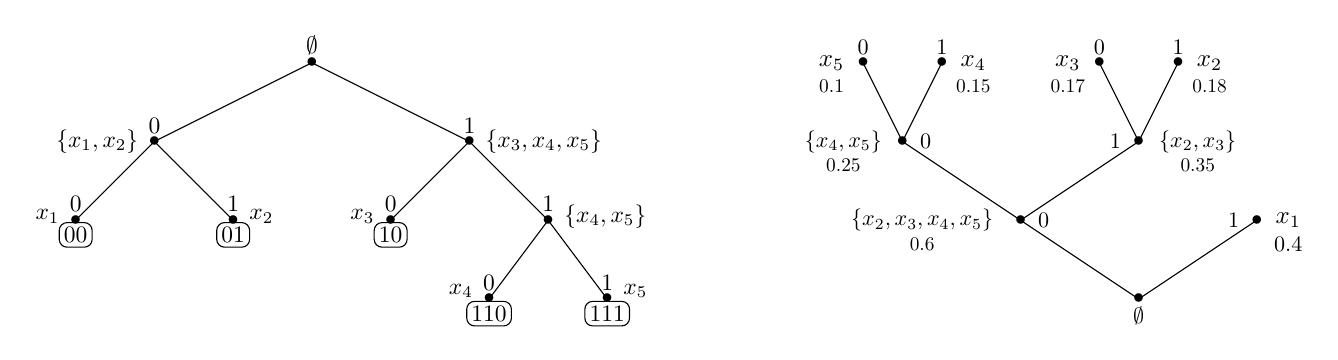
\begin{tikzpicture}%[xscale=3.5,yscale=3]
\shorthandoff{>}
%
% Codigo de Fano
\begin{scope}
\draw(0,0) node[scale=.8]{$\bullet$} node[above,scale=.85]{$\emptyset$};
%
% -----
%
\draw (0,0) -- (-2,-1) node[scale=.8]{$\bullet$} node[above,scale=.85]{$0$};
\draw (-2.1,-1) node[left,scale=.85]{$\{ x_1,x_2\}$};
%
\draw (0,0) -- (2,-1) node[scale=.8]{$\bullet$} node[above,scale=.85]{$1$};
\draw(2.1,-1) node[right,scale=.85]{$\{ x_3,x_4,x_5\}$};
%
% -----
%
\draw (-2,-1) -- (-3,-2) node[scale=.8]{$\bullet$} node[above,scale=.85]{$0$}
node[inner sep=2pt,outer sep=1pt,draw=black,below,scale=.85,rounded corners=1mm]{$00$};
\draw (-3.1,-1.95) node[left,scale=.85]{$\boldsymbol{x_1}$};
%
\draw (-2,-1) -- (-1,-2) node[scale=.8]{$\bullet$} node[above,scale=.85]{$1$}
node[inner sep=2pt,outer sep=1pt,draw=black,below,scale=.85,rounded corners=1mm]{$01$};
\draw (-.9,-1.95) node[right,scale=.85]{$\boldsymbol{x_2}$};
%
\draw (2,-1)-- (1,-2) node[scale=.8]{$\bullet$} node[above,scale=.85]{$0$}
node[inner sep=2pt,outer sep=1pt,draw=black,below,scale=.85,rounded corners=1mm]{$10$};
\draw (.9,-1.95) node[left,scale=.85]{$\boldsymbol{x_3}$};
%
\draw (2,-1)-- (3,-2) node[scale=.8]{$\bullet$} node[above,scale=.85]{$1$};
\draw (3.1,-1.95) node[right,scale=.85]{$\{ x_4 , x_5 \}$};
%
% -----
%
\draw (3,-2)-- (2.25,-3) node[scale=.8]{$\bullet$} node[above,scale=.85]{$0$}
node[inner sep=2pt,outer sep=1pt,draw=black,below,scale=.85,rounded corners=1mm]{$110$};
\draw (2.15,-2.9) node[left,scale=.85]{$\boldsymbol{x_4}$};
%
\draw (3,-2)-- (3.75,-3) node[scale=.8]{$\bullet$} node[above,scale=.85]{$1$}
node[inner sep=2pt,outer sep=1pt,draw=black,below,scale=.85,rounded corners=1mm]{$111$};
\draw (3.85,-2.9) node[right,scale=.85]{$\boldsymbol{x_5}$};
\end{scope}
%
%
% Codigo de Huffman
\begin{scope}[xshift=12cm]
\draw (-5,0) node[scale=.8]{$\bullet$} node[above,scale=.8]{$0$}
-- (-4.5,-1) node[scale=.8]{$\bullet$} node[right,scale=.8]{$\:\: 0$}
-- (-4,0) node[scale=.8]{$\bullet$} node[above,scale=.8]{$1$};
\draw(-5.4,0) node[scale=.9]{$\boldsymbol{x_5}$};
\draw(-5.4,-.3) node[scale=.7]{$0.1$};
\draw(-3.6,0) node[scale=.9]{$\boldsymbol{x_4}$};
\draw(-3.6,-.3) node[scale=.7]{$0.15$};
\draw(-5.25,-1) node[scale=.8]{$\{x_4,x_5\}$};
\draw(-5.25,-1.3) node[scale=.7]{$0.25$};
%
% -----
%
\draw (-2,0) node[scale=.8]{$\bullet$} node[above,scale=.8]{$0$}
-- (-1.5,-1) node[scale=.8]{$\bullet$} node[left,scale=.8]{$1\:\: $}
-- (-1,0) node[scale=.8]{$\bullet$} node[above,scale=.8]{$1$};
\draw(-2.4,0) node[scale=.9]{$\boldsymbol{x_3}$};
\draw(-2.4,-.3) node[scale=.7]{$0.17$};
\draw(-.6,0) node[scale=.9]{$\boldsymbol{x_2}$};
\draw(-.6,-.3) node[scale=.7]{$0.18$};
\draw(-.75,-1) node[scale=.8]{$\{x_2,x_3\}$};
\draw(-.75,-1.3) node[scale=.7]{$0.35$};
%
% -----
%
\draw (-4.5,-1) -- (-3,-2) node[scale=.8]{$\bullet$} node[right,scale=.8]{$\:\: 0$} -- (-1.5,-1);
\draw(-4.25,-2) node[scale=.8]{$\{x_2,x_3,x_4,x_5\}$};
\draw(-4.25,-2.3) node[scale=.7]{$0.6$};
%
% -----
%
\draw (-3,-2) -- (-1.5,-3) node[scale=.8]{$\bullet$} node[below,scale=.8]{$\emptyset$}
-- (0,-2) node[scale=.8]{$\bullet$} node[left,scale=.8]{$1\:\:$};
\draw(.4,-2) node[scale=.9]{$\boldsymbol{x_1}$};
\draw(.4,-2.3) node[scale=.8]{$0.4$};
\end{scope}
\end{tikzpicture} \end{center}
%
\leyenda{Construcci\'on de  un c\'odigo binario  sobre $\C =  \{0 \, , \,  1 \}$
  asociado al  vector de  probabilidad $p_X  = \big[ 0.4  \quad 0.18  \quad 0.17
  \quad 0.15 \quad 0.1 \big]^t$ sobre  el arbol de Kraft.  En este caso, $H_2(X)
  \approx 2.1514$\ (a):  Enfoque de Fano, saliendo de la  ra\'iz.  En cada nudo,
  se  menciona   el  conjunto  de  s\'imbolos   que  va  a   tener  el  c\'odigo
  correspondiente  (en negro  cuando  es un  solo  s\'imbolo).  Se  pasa de  una
  profundez  a la  otra  dividiendo los  conjunto  en sub-conjuntos  a lo  m\'as
  equiprobables.  Esta construcci\'on  da el  c\'odigo  \ $c^\fa(x_1)  = 00,  \:
  c^\fa(x_2) = 01, \: c^\fa(x_3) = 10, \: c^\fa(x_4) = 110, \: c^\fa(x_5) = 111$
  \ de  largo promedio \ $L\left(  c^\fa \right) =  2.25$.  \ \ (b):  Enfoque de
  Huffman, saliendo de las hojas.   En cada nudo, se menciona el correspondiente
  (i) conjunto de s\'imbolos, (ii) $\cod_i$ de esta profundez/posici\'on, (iii)
  la probabilidad  asociada al  conjunto.  Se  pasa de una  profundez a  la otra
  juntando  los conjuntos  menos  probables en  sobre-conjuntos.   En negro  son
  indicados los s\'imbolos simples: van a tener el c\'odigo agregando los de los
  nudos yendo de la ra\'iz hasta  las hojas.  Esta construcci\'on da el c\'odigo
  \ $c^\huf(x_1) = 1, \: c^\huf(x_2) = 011, \: c^\huf(x_3) = 010, \: c^\huf(x_4)
  = 001, \: c^\huf(x_5) = 000$ \ de largo promedio \ $L^\opt = 2.2$.}
%
\label{Fig:SZ:FanoHuffmanCodes}
\end{figure}


Se notar\'a  de que, tratando  de una fuente  \ $\{ X_t  \}_{t \in \Zset}$  \ de
variables independientes,  se puede  codificar la fuente  con un  largo promedio
arbitrariamente cerca  de $H_d(X)$.   El principio es  de considerar  vectores \
$\begin{bmatrix} X_1 & \cdots &  X_n \end{bmatrix}^t$ \ viviendo sobre \ $\X^n$,
llamado {\it extensi\'on de orden $n$ de la fuente}, con un c\'odigo descifrable
(o libre de  prefijo) de esta extensi\'on; es llamado  {\it codificaci\'on de la
  extensi\'on  de  la  fuente}  pero  no  es  necesariamente  una  extension  de
$c$. As\'i, \ $H_d(X_1 , \ldots ,  X_n) \le L^{\opt,n} < H_d(X_1 , \ldots , X_n)
+ 1$, es decir, de la independencia,
%
\[
H_d(X)  \:  \le \:  \frac{L^{\opt,n}}{n}  \: <  \:  H_d(X)  + \frac{1}{n}  \quad
\mbox{por s\'imbolo}
\]
%
(ver  tambi\'en~\cite[cap. 13,  teorema de  Shannon]{Rio07}). Fijense  que  si \
$\displaystyle   \lim_{n   \to  \infty}   \frac{L^{\opt,n}}{n}   \to  H(X)$,   \
$\frac{L^{\opt,n}}{n}$ \ no  es necesariamente decreciente con respeto  a \ $n$.
Eso  es descrito  figura Fig.~\ref{Fig:SZ:CodigosExtensiones}.   Lo  mismo puede
ocurir con el  c\'odigo de Shannon \SZ{y lo de Fano}.  Adem\'as, el cardinal del
alfabeto  extendido $\X^n$  crece exponencialmente  con $n$,  lo que  no permite
elegir un $n$ muy grande.

\begin{figure}[h!]
%
\begin{center} \begin{tikzpicture}
\shorthandoff{>}
%
%Axes
%\pgfmathsetmacro{\Hd}{-.34*log2(.34)-.66*log2(.66)}; % entropia para p = [.34 .66]
%
\draw[>=stealth,->] (.9,0)--(15.5,0) node[right]{\small $n$};
\draw[>=stealth,->] (1,-.1)--(1,2.5)
node[above,scale=.65]{$\displaystyle \frac{L^{\opt,n}}{n} - H_d(X)$};
\foreach \k in {1,...,15} {\draw (\k,0)--(\k,-.1) node[below,scale=.7]{\k};}
\draw (1,2)--(.9,2) node[left,scale=.7]{$1-H_d(X)$};
%
\draw[thin,color=gray!70] plot[mark=*,mark size=1.25, mark options={black}]
file {Data_SZ/Loptn_p033_libro.txt};
%\draw[thin,dashed] (-.1,\dec) node[left]{\small $H_d(X)$} --(12,\dec);
%\draw[thin,dashed] plot [domain=2:13,samples=100] (\x,{50/\x});
% ATTENTION, trace de (L-Hd) normalise puis double pour une question de lisibilite
\end{tikzpicture}
 \end{center}
%
\leyenda{$\frac{L^{\opt,n}}{n}-H_d(X)$  (puntos),   diferencia  entre  el  largo
  promedio \'optimo por s\'imbolo de las  extensiones \ $\X^n$ \ de orden $n$ de
  la fuente $\X$ y la cota inferior en funci\'on de $n$. La linea llena en grise
  sirve como gu\'ia. En esta ilustraci\'on se usa el ejemplo lo m\'as simple con
  \ $d = 2$ \ y \ $p = [0.33 \quad 0.67]^t$.}
%
\label{Fig:SZ:CodigosExtensiones}
\end{figure}

\

Para  codificar una  fuente, que  se haga  el c\'odigo  \'optimo de  Fano,  o de
Shannon,  hace  falta  usar  la  distribuci\'on de  probabilidad  de  la  fuente
$X$. Pr\'acticamente, es usual que no se la tiene. Frecuentemente, es estimada a
partir de datos,  o, dicho de otra manera, se  c\'odifica con una distribuci\'on
que no es la distribuci\'on verdadera de la fuenta. Una pregunta que surge es de
conocer lo que se pierde usando una distribuci\'on no adaptada (o ``falsa''). La
respuesta general  no es obvia, pero  tratando del c\'odigo de  Shannon se puede
contestar:

\begin{teorema}[C\'odigo falso de Shannon]
\label{Teo:SZ:CodigoFalsoShannon}
%
  Sea $c^\sh(p)$  el c\'odigo de Shannon sobre  el alfabeto c\'odigo \  $\C = \{
  \cod_1 ,  \ldots , \cod_d \}$ asociado  a la distribuci\'on $p$.   Sea $X$ \
  fuente sobre  \ $\X$, de distribuci\'on \  $p_X$ \ y \  $q$ una distribuci\'on
  cualquiera  (ej.  estimada  de  $p_X$ presupuesta\ldots).   Entonces el  largo
  promedio \ $L_{c^\sh(q)}$ \ del c\'odigo \ $c^\sh(q)$ \ aplicado a la fuente \
  $X$ \ satisface las desigualdades siguientes
  %
  \[
  H_d(p_X) +  D_{\mathrm{kl},d}\left( \left.  p_X \right\| q  \right) \:  \le \:
  L_{c^\sh(q)} \: < \: H_d(p_X)  + D_{\mathrm{kl},d}\left( \left. p_X \right\| q
  \right) + 1.
  \]
\end{teorema}
%
\begin{proof}
  Por definici\'on,
  \[
  L_{c^\sh}(q) = \sum_{x \in X} p_X(x) \, \Big\lceil\! -\log_d q(x) \Big\rceil.
  \]
  %
  La desigualdad viene de  \ $a \le \lceil a \rceil < a +  1$ \ y escribiendo $-
  p_X \log_d q = - p_X \log_d p_X + p_X \log \left( \frac{p_X}{q} \right)$.
\end{proof}
%
Olvidando el  posible extra dit (pensar  a la c\'odification  por bloques), este
teorema  da  una  interpretaci\'on  operacional  a  la  entrop\'ia  relativa,  o
divergencia  de  Kullback-Leibler.   Esta  cantidad  cuantifica  la  perdida  en
t\'ermino de largo  promedio codificando con una distribuci\'on  falsa. Dicho de
otra manera,  usando $q$  en lugar de  $p_X$, se  usa la informaci\'on  de $p_X$
porque se  c\'odifica la fuente $X$,  pero suponiendo la  distribuc\'ion $q$, se
piedre lo  que representa la  informaci\'on relativa de  $p_X$ con respeto  a la
referencia (distribuci\'on supuesta) $q$.

\

Existen varios otros  modos de codificar s\'imbolos. En  particular, con la meta
de transmitir los s\'imbolos codificados  en un canal de comunicaci\'on, a veces
no  es oportuno  de compresar  drasticamente  el mensaje.   Existen por  ejemplo
codificaciones que permiten una correcci\'on  de error en la recepci\'on. Pueden
tomar  en  cuenta  las   caracteristicas  del  canal  de  transmisi\'on.   Estas
consideraciones  van m\'as  all\'a de  la  ilustraci\'on de  esta secci\'on.  El
lector puede referirse a~\cite{Ber74, Gal78, Say03, CovTho06, Rio07} entre otros
para tener m\'as detalles sobre varios esquemas de codificaci\'on/compresi\'on.

% R.  M.  Fano.  Class  notes  for Transmission  of  Information,  course  6.574
% (Technical Report). MIT, Cambridge, MA, 1952

%\SZ{Dire  un mot  sur  le codage  canal.   Cf avec  la  distribucion optimale  /
%  capacite cf. Elias 1954 - error free coding, Elias 1955 - error noisy channel,
%  Elias 57  - list  for decoding noisy  channels, Berlekamp (serie  papiers cles
%  dans les premiers).}

% ================================= Gaz perfecto

\subseccion{Gas perfecto}
\label{Ssec:SZ:GasPerfecto}

En el marco del gas perfecto

\SZ{Va donner un lien avec Boltzmann}


\

\SZ{Feder  Merhav  IT'94  et  lien  avec  discrimination;  Vacisek  en  test  de
  Gaussianite et cf plus loin avec generalises Gok75 etc}
